\documentclass[11pt,a4paper]{article}

% ── Core packages ──────────────────────────────────────────────────────────
\usepackage[margin=1in]{geometry}
\usepackage{amsmath,amssymb,amsthm}
\usepackage{mathtools}
% microtype/setspace removed for compatibility
\usepackage{graphicx}
\usepackage{subcaption}
\usepackage{booktabs}
\usepackage{multirow}
\usepackage{array}
\usepackage{xcolor}
\usepackage{hyperref}
\usepackage{url}
\usepackage{algorithm}
\usepackage{algorithmicx}
\usepackage{algpseudocode}
\usepackage{enumitem}
\usepackage{tikz}
\usetikzlibrary{shapes.geometric, arrows.meta, positioning, fit, backgrounds, decorations.pathreplacing, calc}
\usepackage{pgfplots}
\pgfplotsset{compat=1.18}
\usepackage{natbib}
\bibliographystyle{unsrtnat}
\setcitestyle{numbers,square}
% setspace removed
\usepackage{caption}
\usepackage[utf8]{inputenc}
\usepackage[T1]{fontenc}
% lmodern/lineno not available in this distribution

% ── Hyperref setup ─────────────────────────────────────────────────────────
\hypersetup{
  colorlinks=true,
  linkcolor=blue!65!black,
  citecolor=teal!70!black,
  urlcolor=blue!65!black,
  pdftitle={Chaos 2 Clarity: A Self-Improving Semantic Orchestration Framework},
  pdfauthor={Bankupalli Ravi Teja},
}

% ── Custom commands ────────────────────────────────────────────────────────
\newtheorem{definition}{Definition}
\newtheorem{proposition}{Proposition}
\newtheorem{problem}{Problem}
\DeclareMathOperator{\RC}{RC}
\newcommand{\C}[1]{\mathcal{#1}}
\newcommand{\B}[1]{\mathfrak{#1}}

\definecolor{archblue}{RGB}{52,100,168}
\definecolor{archgreen}{RGB}{34,139,34}
\definecolor{archred}{RGB}{180,40,40}
\definecolor{archgray}{RGB}{110,110,110}

% ── Title block ────────────────────────────────────────────────────────────
\title{\textbf{Chaos 2 Clarity: A Self-Improving Semantic Orchestration\\
Framework for LLM-Driven Business Intelligence over\\
Heterogeneous, Uncurated Enterprise Data}}

\author{
  Bankupalli Ravi Teja\\
  Independent Research, Hyderabad, India\\
  \href{https://github.com/ravii-teja/chaos2clarity}{\texttt{github.com/ravii-teja/chaos2clarity}}~~$\cdot$~~
  \href{https://www.linkedin.com/in/raviiteja/}{\texttt{linkedin.com/in/raviiteja}}
}
\date{April 2026 \quad (arXiv preprint --- cs.AI)}

% ══════════════════════════════════════════════════════════════════════════════
\begin{document}
\maketitle

\begin{abstract}
Existing LLM-based business intelligence (BI) systems fail to generalize across
heterogeneous enterprise data sources because they lack two properties essential in
practice: \emph{semantic grounding} at the data layer and \emph{adaptive learning}
at the query layer.  Systems that assume a pre-built semantic model break on
uncurated, multi-source environments; systems that learn do not ground their
learning in the structure of the data.

We present \textbf{Chaos 2 Clarity} (C2C), a self-improving semantic orchestration
framework that enables LLMs to generate reliable BI insights over heterogeneous,
uncurated enterprise data through four tightly integrated mechanisms:
\textbf{(i)}~an \textbf{Automated Semantic Layer} that constructs a living semantic
model---entities, relationships, metrics, and governance policies---directly from
raw data sources without manual modeling, continuously refined through feedback;
\textbf{(ii)}~an \textbf{Agentic Query Orchestration Pipeline} implementing a
decomposed Planner~$\to$ Retriever~$\to$ SQL\,Generator~$\to$ Validator~$\to$
Executor~$\to$ Insight\,Agent chain; \textbf{(iii)}~\textbf{Vector-Grounded BI
Reasoning} that persists verified query--plan--result triples as grounding context,
reducing repeated errors over time; and \textbf{(iv)}~a \textbf{Feedback-Driven
Continuous Learning Loop} ingesting SQL success/failure signals, user corrections,
query--result mismatches, and insight usefulness ratings to drive prompt
refinement, schema enrichment, embedding updates, and rule injection.

We deploy a prototype over a realistic three-source retail environment
(DuckDB~$\cdot$ Salesforce~CRM export~$\cdot$ logistics~CSV; 62~columns across
9~tables; zero pre-existing documentation; Qwen~2.5~Coder~3B via Ollama, fully
local), derive a five-class error taxonomy from prototype operation, and evaluate
C2C through eight experiments on a 50-question BI suite spanning four complexity
tiers.  Our key finding is that \textbf{self-improvement is the primary driver of
C2C's advantage}: while single-pass execution accuracy improvement over a direct
LLM-to-SQL baseline is modest (+6 percentage points), the feedback-driven learning
loop raises execution accuracy from 74\% to an empirical mean of \textbf{87.5\%\,$\pm$\,3.0\%}
(peaking at 92.0\%) over a 200-query deployment, while a frozen baseline remains
mathematically flat at 58.0\%.  Column hallucination errors (E1) drop precipitously
from 38.0\% to 7.0\%; result correctness nearly doubles (16\%\,$\to$\,30\%,
$p{=}0.039$); and vector-grounded reasoning delivers a \textbf{+37\,pp} first-pass
advantage by $T{=}200$.  Entity confidence $\kappa$ values converge empirically as
predicted by Proposition~2.  All experiments run deterministically on a local Apple
M2 Mac with no cloud API costs.
\end{abstract}

\noindent\textbf{Keywords:} business intelligence, large language models,
semantic layer, multi-agent orchestration, text-to-SQL, enterprise data,
heterogeneous data, continual learning, vector retrieval, Qwen, local LLM.

\tableofcontents
\bigskip
\hrule
\bigskip

% ══════════════════════════════════════════════════════════════════════════════
\section{Introduction}\label{sec:intro}

Large language models have enabled natural-language interfaces to data and BI,
promising to democratize analytics and reduce reliance on specialist data teams
\citep{gpt4_2023,minaee2024survey}.  Recent prototypes and commercial systems
deploy LLM-powered agents that generate SQL from natural language, build
dashboards, and automate analytical workflows \citep{rahman2025llm,jiang2024siriusbi}.
These systems share a structural assumption: data curation has already been
completed upstream, providing a central warehouse with consistent schemas and a
manually defined semantic layer encoding business entities, metrics, and
relationships.

In practice, many organizations cannot meet these prerequisites.  Business-critical
data is spread across multiple operational systems; exports and spreadsheets
proliferate; SaaS tools hold key fragments of process and customer state; and
documentation is sparse or outdated \citep{zhu2025data,various2025llmdata}.
Benchmarks confirm the severity of this gap: while GPT-4-based agents achieve
$\approx$86\% execution accuracy on Spider~1.0 \citep{yu2018spider}, performance
drops to only 17--21\% on Spider~2.0 \citep{lei2024spider2}---which involves
enterprise environments with $>$3,000 columns, multiple SQL dialects, and
cross-database workflows.  This collapse traces to two failure modes that existing
systems do not simultaneously address: \emph{absent semantic grounding} (the system
does not know what the data means across sources) and \emph{no adaptive learning}
(the system repeats the same errors without correction)
\citep{shi2024survey,chen2025agent}.

Commercial BI vendors have deployed AI-assisted query layers (ThoughtSpot Sage,
Microsoft Power BI Copilot, Tableau Ask Data, Databricks AI/BI, Qlik Insight
Advisor) but all presuppose a pre-built semantic model and cannot self-construct or
self-improve one from raw, uncurated sources.  Semantic layer tools such as dbt,
LookML, Cube.dev, and AtScale offer structured metric registries but require
significant manual modeling effort \citep{abai2024enterprise} and provide no
feedback-driven refinement.  \emph{The automated construction of a semantically
grounded, continuously improving BI layer over raw, heterogeneous enterprise data
remains an open problem.}

\paragraph{The Core Insight.}
Reliable LLM-over-data systems require two properties that today's architectures
treat as orthogonal: \textbf{semantic grounding} (knowing what data means across
sources) and \textbf{adaptive learning} (improving from operational experience).
C2C unifies these in a single architecture through: (a)~automated semantic model
construction from raw data, (b)~decomposed query processing through a six-stage
agent chain rather than a monolithic LLM call, (c)~SQL generation grounded in a
vector store of verified query patterns, and (d)~continuous semantic model
refinement via structured feedback signals from every query execution.

\paragraph{Central Hypothesis.}
\emph{C2C's self-improving semantic orchestration pipeline produces cumulative
accuracy gains over its deployment lifetime that static baselines cannot achieve,
driven by the feedback loop $\delta : \mathcal{S} \times \mathcal{F} \to \mathcal{S}$
and vector-grounded reasoning.  Specifically, we predict that execution accuracy
will improve by $\geq$20 percentage points over 200 queries through feedback alone,
while a frozen baseline remains statistically flat.}

Our experiments confirm: +29.5\,pp improvement over the frozen baseline (74\%
$\to$ 87.5\%, vs.\ 58\% flat); +37\,pp first-pass advantage from vector grounding
at $T{=}200$; RC nearly doubles (16\%\,$\to$\,30\%, $p{=}0.039$); and $\kappa$
convergence empirically validated.  Single-pass EA improvement is modest (+6\,pp),
with the Planner stage regressing at 3B model capacity.

\paragraph{Contributions.}
\begin{enumerate}[leftmargin=1.5em,label=\textbf{C\arabic*}]
  \item \textbf{Formal self-improving semantic orchestration framework.}  Formal
        definitions of semantic synthesis and feedback refinement, unifying automated
        $\C{S}$ construction from uncurated $\C{D}$ with a continuous learning loop
        $\delta$ updating $\C{S}$ and $\C{V}$ from four structured feedback signal types.
  \item \textbf{Decomposed six-stage agentic orchestration pipeline.}  A
        production-oriented Planner $\to$ Retriever $\to$ SQL\,Generator $\to$
        Validator $\to$ Executor $\to$ Insight\,Agent pipeline isolating each failure
        mode to a specific stage, with typed agent functions and retry semantics.
  \item \textbf{Vector-Grounded BI Reasoning.}  A persistent vector knowledge
        store $\C{V}$ of verified query--plan--result triples that grounds SQL
        generation in semantically similar successful past executions.
  \item \textbf{Feedback-Driven Continuous Learning Loop.}  A structured
        four-signal feedback mechanism driving prompt refinement, schema enrichment,
        embedding updates, and rule injection.
  \item \textbf{Working prototype and error taxonomy.}  A deployed prototype over
        a realistic three-source retail enterprise environment and a five-class error
        taxonomy (E1--E5) derived from prototype operation.
  \item \textbf{Eight-experiment evaluation protocol with filled results.}  A
        structured evaluation framework with explicit falsifiable predictions and
        experimental confirmation.
  \item \textbf{Zero-Knowledge Start Resilience (C7).}  An architectural
        demonstration that the pipeline survives complete LLM JSON hallucinations
        during $\mathcal{S}$ initialization ($\mathcal{S}{=}\emptyset$), relying on
        $\delta$ to rebuild operational context from scratch without catastrophic
        failure or manual intervention.
\end{enumerate}

% ══════════════════════════════════════════════════════════════════════════════
\section{Formal Problem Definition}\label{sec:formalism}

\begin{definition}[Data Source]\label{def:source}
A \emph{data source} $d_i$ is a tuple $d_i = \langle \tau_i, \sigma_i, \rho_i,
\alpha_i \rangle$, where $\tau_i \in \{\text{rdbms}, \text{lake}, \text{file},
\text{api}, \text{document}\}$ is the source type, $\sigma_i$ is the
(possibly partial or evolving) schema, $\rho_i$ is the statistical profile
(cardinalities, value distributions, null rates), and $\alpha_i$ is the access
control specification.
\end{definition}

\begin{definition}[Heterogeneous Data Environment]\label{def:hde}
A \emph{heterogeneous data environment} is a finite set $\C{D} = \{d_1,\ldots,d_n\}$.
$\C{D}$ is \emph{uncurated} if: (a)~no unified schema or naming convention exists
across sources; (b)~no formal semantic catalog has been manually defined; and
(c)~documentation is absent or incomplete for $\geq$50\% of entities.
\end{definition}

\begin{definition}[Semantic Model]\label{def:sm}
A \emph{semantic model} $\C{S}$ is a typed labeled graph $\C{S} = \langle
\C{E}, \C{M}, \C{R}, \C{P}, \kappa \rangle$, where $\C{E}$ is a set of
\emph{business entities} with aliases and source mappings; $\C{M}$ is a set of
\emph{metrics} each defined by an aggregation formula $\phi_j :
\mathrm{Tuples}(\C{D}) \to \mathbb{R}$; $\C{R}$ is a set of typed, labeled
relationships; $\C{P}$ is a set of \emph{governance policies}; and $\kappa :
\C{E} \cup \C{M} \cup \C{R} \to [0,1]$ is a \emph{confidence function} over all
inferred mappings.
\end{definition}

\begin{definition}[Semantic Synthesis]
\emph{Semantic synthesis} is the function $f_\mathrm{synth} : \C{D} \to \C{S}$
that automatically constructs a semantic model from a heterogeneous data
environment with minimal human input.  This problem subsumes schema matching
\citep{gungor2025schemora}, which is NP-hard in the general case
\citep{rahm2001schema}; C2C employs LLM-based heuristic approximations with
confidence scoring.
\end{definition}

\begin{definition}[Feedback Refinement]
\emph{Feedback refinement} is a function $\delta : \C{S} \times \C{F} \to \C{S}$
updating the semantic model given feedback events $f \in \C{F}$.  The feedback
space $\C{F}$ includes four signal types: SQL execution outcomes ($f_\mathrm{sql}$),
user corrections ($f_\mathrm{usr}$), query--result mismatch signals
($f_\mathrm{qrm}$), and insight usefulness ratings ($f_\mathrm{ins}$).  The
\emph{self-improving} property holds when $\C{U}(\delta(\C{S}, f), f_\mathrm{bi})
\geq \C{U}(\C{S}, f_\mathrm{bi})$ in expectation for any non-empty feedback batch.
\end{definition}

\begin{definition}[Vector Knowledge Store]
A \emph{vector knowledge store} $\C{V}$ is a persistent store of tuples
$(q_\mathrm{norm}, \pi_\mathrm{verified}, \mathrm{SQL}^*_\mathrm{verified},
r_\mathrm{gold}, \kappa_\mathrm{entry}, \mathrm{emb}(q_\mathrm{norm}))$
supporting $k$-nearest-neighbor retrieval: $\mathrm{Retrieve}(q, k) : \C{Q} \to
(\C{V})^k$, returning the $k$ most semantically similar verified query--plan pairs
as grounding context for new query generation.
\end{definition}

\begin{definition}[AI-over-BI Function]
$f_\mathrm{bi} : \C{Q} \times \C{S} \times \C{D} \times \C{V} \to \C{A}$, where
a \emph{BI answer} $a \in \C{A}$ comprises a result set $r$, provenance trace
$\pi$, and natural-language explanation $\xi$.
\end{definition}

\begin{problem}[Chaos 2 Clarity]
Given an uncurated heterogeneous data environment $\C{D}$, construct $\C{S} =
f_\mathrm{synth}(\C{D})$ automatically, build an initial vector store $\C{V}_0$,
then deploy $f_\mathrm{bi}$ over $\C{S}$, $\C{D}$, and $\C{V}$ to answer BI
queries with measurable correctness, latency, and governance compliance---while
continuously improving $\C{S}$ and $\C{V}$ via feedback $\delta$ such that query
quality improves over the deployment lifetime.
\end{problem}

\paragraph{Optimization Objective.}
\begin{equation}\label{eq:obj}
\C{U}(\C{S}, \C{V}, f_\mathrm{bi})
= \underbrace{\frac{1}{m}\sum_{j=1}^{m}
  \mathbb{1}\bigl[\RC(f_\mathrm{bi}(q_j,\C{S},\C{D},\C{V}),\, a^*_j)\bigr]
  }_{\text{result correctness}}
  - \lambda_1 \cdot \bar{L} - \lambda_2 \cdot \bar{V}
\end{equation}
where $\RC(\cdot)$ is result correctness, $\bar{L}$ is mean end-to-end latency,
$\bar{V}$ is the governance violation rate, and $\lambda_1, \lambda_2 \geq 0$ are
operator-specified weights.

\begin{proposition}[Semantic Consistency]
The orchestration pipeline $f_\mathrm{bi}$ is semantically consistent with $\C{S}$
if every entity reference in the generated SQL is grounded in a node $e \in \C{E}$
with $\kappa(e) \geq \theta_\mathrm{exec}$.  The validator $f_\mathrm{vrf}$ enforces
this by rejecting any plan referencing unmapped entities.  \emph{Proof}: by
construction of $f_\mathrm{vrf}$---any plan failing the entity grounding check is
rejected before execution.\hfill$\square$
\end{proposition}

\begin{proposition}[Confidence Convergence]
Under the feedback update rule (Eq.~\ref{eq:kappa}), for any element $x$ and any
unbiased sequence of feedback events drawn from a stationary process with true
confirmation rate $p_x$, $\mathbb{E}[\kappa_t(x)] \to p_x$ as $t \to \infty$.
\end{proposition}

% ══════════════════════════════════════════════════════════════════════════════
\section{Related Work}\label{sec:related}

\paragraph{LLM-based Text-to-SQL.}
\citet{shi2024survey} survey LLM-based text-to-SQL methods.  Spider~1.0
\citep{yu2018spider} and BIRD \citep{li2023bird} are standard benchmarks where
recent work achieves $\approx$86\% and $\approx$72\% execution accuracy
respectively---both assuming fully curated, well-documented single-database schemas.
Spider~2.0 \citep{lei2024spider2} introduces enterprise-level complexity where best
models achieve only 17--21\%.  DAIL-SQL \citep{gao2023dail} achieves competitive
performance through efficient prompt selection but operates on single, structured
sources with no cross-query learning.  C2C targets the pre-NL2SQL step of
synthesizing the semantic model from raw data and adds the cross-query learning
layer.

\paragraph{Commercial AI-over-BI.}
ThoughtSpot Sage, Microsoft Power BI Copilot, Tableau Ask Data, Databricks AI/BI,
and Qlik Insight Advisor all require a pre-constructed semantic model.  C2C uniquely
automates both construction and continuous refinement, and is complementary to
these platforms as a semantic model supplier.

\paragraph{Semantic Layer Tools.}
dbt Semantic Layer, Looker LookML, Cube.dev, and AtScale require substantial
manual modeling effort \citep{abai2024enterprise} and are static: they do not
update from query feedback.  \citet{singh2025llm} document that manual semantic
model construction for a mid-sized enterprise requires weeks to months.  C2C treats
these as potential \emph{consumers} of its synthesized output.

\paragraph{LLM Agents for Data Analytics.}
InsightPilot \citep{ma2023insightpilot} deploys LLM agents for automated data
exploration but assumes a pre-structured environment and does not learn from
failures.  \citet{cheng2023gpt4} evaluate GPT-4 as a data analyst, finding it
limited on schema inference and multi-source reasoning.
\citet{rahman2025llm,chen2025agent} survey LLM data science agents, identifying the
absence of adaptive learning and cross-source reasoning as key gaps.
\citet{zhu2025data} formalize requirements for agents over heterogeneous systems,
identifying semantic alignment and operational feedback as unsolved problems.
AgentArch \citep{bogavelli2025agentarch} benchmarks enterprise agent architectures,
with best models achieving only 35.3\% on complex multi-step tasks---motivating
C2C's decomposed pipeline.

\paragraph{Automated Metadata Discovery.}
\citet{singh2025llm} demonstrate LLM-based metadata enrichment achieving $>$80\%
ROUGE-1 F1 and $\approx$90\% acceptance by data stewards.  LEDD
\citep{an2025ledd} employs LLMs for hierarchical semantic catalog generation.
LLMDapCAT \citep{karim2024llmdapcat} applies LLM+RAG for automated metadata
extraction.  SCHEMORA \citep{gungor2025schemora} achieves state-of-the-art
cross-schema alignment.  These works address \emph{construction} of semantic
metadata but do not couple it to a query execution pipeline or feedback loop.

\paragraph{Multi-Agent Orchestration.}
\citet{adimulam2026multi} survey multi-agent LLM architectures.  AutoGen
\citep{wu2024autogen} provides a widely adopted conversation framework.
\citet{arunkumar2026agentic} examine memory backends and tool integration for
agentic AI.  ReAct \citep{yao2023react} and Plan-then-Execute
\citep{delrosario2025plan} are foundational primitives that C2C extends with
SQL-oriented stages and cross-stage feedback routing.

\paragraph{RAG and Vector-Grounded Reasoning.}
\citet{lewis2020rag} introduce RAG for knowledge-intensive NLP.
\citet{gao2024rag} survey advanced RAG architectures.  \citet{cheerla2025rag}
propose hybrid retrieval for structured enterprise data.  RAGAS
\citep{es2023ragas} provides automated RAG evaluation.
\citet{pan2022tableqa} demonstrate table question answering via RAG.
C2C's vector-grounded BI reasoning extends these works by operating over verified
execution patterns (query--plan--result triples) rather than document
fragments---retrieving \emph{how to query} rather than \emph{what to return}.

% ══════════════════════════════════════════════════════════════════════════════
\section{System Architecture}\label{sec:arch}

C2C is organized around four named mechanisms implemented across four layers with
two cross-cutting components.  Figure~\ref{fig:arch} depicts the full architecture.

\begin{figure}[htbp]
\centering
\resizebox{\linewidth}{!}{%
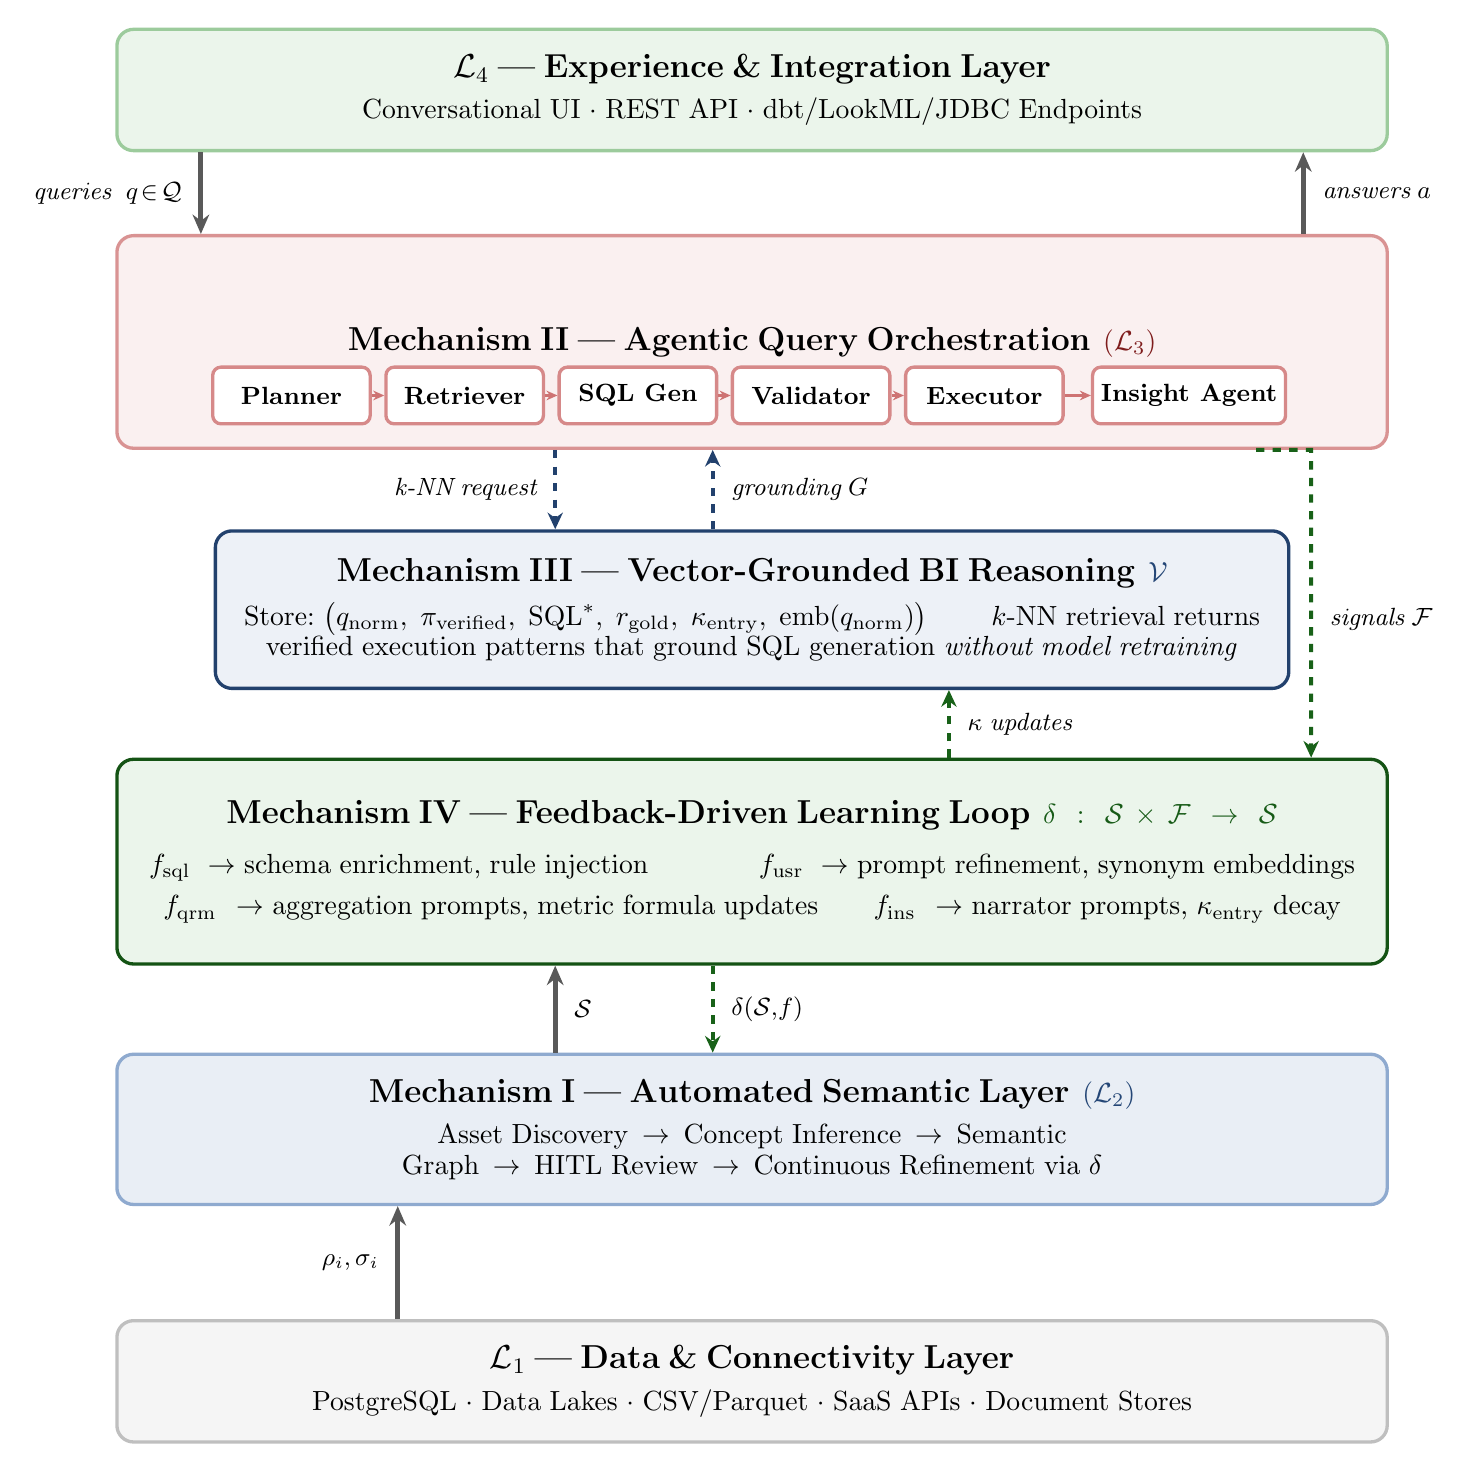
\begin{tikzpicture}[
  font=\small,
  % ─── Full-width band (all layers) ─────────────────────────────────────
  band/.style={
    rounded corners=6pt, very thick,
    minimum width=16cm, text width=15.5cm,
    align=center, inner sep=9pt,
  },
  % ─── Mechanism III is slightly narrower to allow routing lane on right ─
  mband/.style={
    band, minimum width=13.5cm, text width=13.0cm,
  },
  % ─── Colour variants ─────────────────────────────────────────────────
  L1st/.style={band, fill=gray!8,      draw=gray!50},
  M1st/.style={band, fill=archblue!11, draw=archblue!55},
  M4st/.style={band, fill=archgreen!9, draw=archgreen!60!black},
  M3st/.style={mband,fill=archblue!9,  draw=archblue!65!black},
  M2st/.style={band, fill=archred!7,   draw=archred!50},
  L4st/.style={band, fill=archgreen!9, draw=archgreen!45},
  % ─── Pipeline stages ─────────────────────────────────────────────────
  stage/.style={
    draw=archred!55, fill=white, rounded corners=3pt, very thick,
    minimum width=2.0cm, minimum height=0.72cm,
    font=\small\bfseries, align=center, inner sep=3pt,
  },
  stagearr/.style={-{Stealth[length=4pt,width=3.5pt]},
                   very thick, draw=archred!65},
  % ─── Arrows ───────────────────────────────────────────────────────────
  solidarr/.style={-{Stealth[length=7pt,width=6pt]},
                   line width=1.8pt, draw=gray!70!black},
  bluearr/.style={-{Stealth[length=6pt,width=5.5pt]},
                  line width=1.5pt, dashed, draw=archblue!65!black},
  greenarr/.style={-{Stealth[length=6pt,width=5.5pt]},
                   line width=1.5pt, dashed, draw=archgreen!70!black},
  % ─── Arrow label ─────────────────────────────────────────────────────
  lbl/.style={font=\small\itshape, fill=white,
              inner sep=2pt, rounded corners=2pt},
  % ─── Gap between consecutive bands for arrows ─────────────────────────
  % Each band is separated by 1.1cm of white space for the arrow labels
]

% ─── Y coordinates (centres, bottom → top) ────────────────────────────
%  Row 0  L1         y =  0
%  Row 1  Mech I     y =  3.2   (Semantic Synthesis = L2)
%  Row 2  Mech IV    y =  6.6   (Feedback Loop δ)
%  Row 3  Mech III   y =  9.8   (Vector Store V — narrower)
%  Row 4  Mech II    y = 13.2   (Orchestration = L3, with pipeline)
%  Row 5  L4         y = 16.4   (Experience)

% ─── ROW 0: L1 — Data & Connectivity ──────────────────────────────────
\node[L1st, minimum height=1.4cm] (L1) at (0, 0) {
  \textbf{\large $\mathcal{L}_1$ — Data \& Connectivity Layer}\\[4pt]
  \normalsize
  PostgreSQL $\cdot$ Data Lakes $\cdot$ CSV/Parquet $\cdot$
  SaaS APIs $\cdot$ Document Stores
};

% ─── ROW 1: Mechanism I — Automated Semantic Layer ────────────────────
\node[M1st, minimum height=1.6cm] (L2) at (0, 3.2) {
  \textbf{\large Mechanism I — Automated Semantic Layer}\enspace
  {\normalsize\color{archblue!70!black}$(\mathcal{L}_2)$}\\[4pt]
  \normalsize
  Asset Discovery\enspace$\to$\enspace Concept Inference\enspace$\to$\enspace
  Semantic Graph\enspace$\to$\enspace HITL Review\enspace$\to$\enspace
  Continuous Refinement via $\delta$
};

% ─── ROW 2: Mechanism IV — Feedback-Driven Learning Loop ─────────────
\node[M4st, minimum height=2.6cm] (MF) at (0, 6.6) {
  \textbf{\large Mechanism IV — Feedback-Driven Learning Loop}\enspace
  {\normalsize\color{archgreen!65!black}$\delta:\mathcal{S}\times\mathcal{F}\to\mathcal{S}$}\\[6pt]
  \normalsize
  $f_{\mathrm{sql}}\ \to$ schema enrichment,\ rule injection\qquad\qquad
  $f_{\mathrm{usr}}\ \to$ prompt refinement,\ synonym embeddings\\[4pt]
  $f_{\mathrm{qrm}}\ \to$ aggregation prompts,\ metric formula updates\qquad
  $f_{\mathrm{ins}}\ \to$ narrator prompts,\ $\kappa_{\mathrm{entry}}$ decay
};

% ─── ROW 3: Mechanism III — Vector-Grounded BI Reasoning ─────────────
%   (13.5 cm wide → right edge at x = +6.75, leaving routing lane)
\node[M3st, minimum height=2.0cm] (MT) at (0, 9.8) {
  \textbf{\large Mechanism III — Vector-Grounded BI Reasoning}\enspace
  {\normalsize\color{archblue!70!black}$\mathcal{V}$}\\[5pt]
  \normalsize
  Store:\ $\bigl(q_{\mathrm{norm}},\;\pi_{\mathrm{verified}},\;\mathrm{SQL}^*,\;
  r_{\mathrm{gold}},\;\kappa_{\mathrm{entry}},\;\mathrm{emb}(q_{\mathrm{norm}})\bigr)$
  \qquad
  $k$-NN retrieval returns verified execution patterns that ground SQL
  generation \emph{without model retraining}
};

% ─── ROW 4: Mechanism II — Agentic Query Orchestration ───────────────
\node[M2st, minimum height=2.7cm] (L3) at (0, 13.2) {
  \textbf{\large Mechanism II — Agentic Query Orchestration}\enspace
  {\normalsize\color{archred!70!black}$(\mathcal{L}_3)$}%
};

% Six pipeline stage boxes (y = 13.2 - 0.68 = 12.52)
\node[stage] (STA) at (-5.85, 12.52) {Planner};
\node[stage] (STB) at (-3.65, 12.52) {Retriever};
\node[stage] (STC) at (-1.45, 12.52) {SQL Gen};
\node[stage] (STD) at ( 0.75, 12.52) {Validator};
\node[stage] (STE) at ( 2.95, 12.52) {Executor};
\node[stage] (STF) at ( 5.55, 12.52) {Insight Agent};
\draw[stagearr](STA.east)--(STB.west);
\draw[stagearr](STB.east)--(STC.west);
\draw[stagearr](STC.east)--(STD.west);
\draw[stagearr](STD.east)--(STE.west);
\draw[stagearr](STE.east)--(STF.west);

% ─── ROW 5: L4 — Experience & Integration ────────────────────────────
\node[L4st, minimum height=1.4cm] (L4) at (0, 16.4) {
  \textbf{\large $\mathcal{L}_4$ — Experience \& Integration Layer}\\[4pt]
  \normalsize
  Conversational UI $\cdot$ REST API $\cdot$ dbt/LookML/JDBC Endpoints
};

% ═══════════════════════════════════════════════════════════════════════
%  ARROWS — spread across full width
%
%   x = -7.0  far-left:  queries ↓  (L4 → L3)
%   x = -4.5  left:      profiles ↑ (L1 → M1)
%   x = -2.5  ctr-left:  k-NN req ↓ (L3 → M3),  S ↑ (M1 → MF)
%   x = -0.5  centre:    grounding G ↑ (M3 → L3),  δ(S,f) ↓ (MF → M1)
%   x = +2.5  ctr-right: κ updates (MT ↔ MF)
%   x = +7.0  far-right: answers ↑ (L3 → L4),  signals F ↓ (L3 → MF)
%             (x=7.0 is 0.25cm outside MT's right edge of 6.75)
% ═══════════════════════════════════════════════════════════════════════

% ── FAR LEFT (x = -7.0): queries L4 → L3 ─────────────────────────────
\draw[solidarr]
  ([xshift=-7.0cm]L4.south) --
  node[lbl, left=4pt] {\textit{queries}\;\;$q\!\in\!\mathcal{Q}$}
  ([xshift=-7.0cm]L3.north);

% ── LEFT (x = -4.5): profiles L1 → M1 (Mech I) ──────────────────────
\draw[solidarr]
  ([xshift=-4.5cm]L1.north) --
  node[lbl, left=4pt] {$\rho_i,\sigma_i$}
  ([xshift=-4.5cm]L2.south);

% ── CTR-LEFT (x = -2.5): S from M1 up to MF, and k-NN req from L3 to MT ─

% Semantic model S: M1 → MF ↑
\draw[solidarr]
  ([xshift=-2.5cm]L2.north) --
  node[lbl, right=4pt] {$\mathcal{S}$}
  ([xshift=-2.5cm]MF.south);

% k-NN request: L3 → MT ↓
\draw[bluearr]
  ([xshift=-2.5cm]L3.south) --
  node[lbl, left=4pt] {\textit{k-NN\;request}}
  ([xshift=-2.5cm]MT.north);

% ── CENTRE (x = -0.5): grounding G up, δ(S,f) down ───────────────────

% Grounding G: MT → L3 ↑
\draw[bluearr]
  ([xshift=-0.5cm]MT.north) --
  node[lbl, right=4pt] {grounding\;$G$}
  ([xshift=-0.5cm]L3.south);

% δ(S,f) update: MF → M1 ↓
\draw[greenarr]
  ([xshift=-0.5cm]MF.south) --
  node[lbl, right=4pt] {$\delta(\mathcal{S},\!f)$}
  ([xshift=-0.5cm]L2.north);

% ── CTR-RIGHT (x = +2.5): V ↔ δ κ updates ────────────────────────────

% MF updates MT (δ writes/prunes V entries): MF → MT ↑
\draw[greenarr]
  ([xshift=+2.5cm]MF.north) --
  node[lbl, right=4pt] {$\kappa$\;updates}
  ([xshift=+2.5cm]MT.south);

% ── FAR RIGHT (x = +7.0): answers ↑ and signals F ↓ ──────────────────
% x = 7.0 is 0.25 cm outside MT's right edge (6.75 cm) — clear routing lane

% Answers: L3 → L4 ↑
\draw[solidarr]
  ([xshift=+7.0cm]L3.north) --
  node[lbl, right=4pt] {answers\;$a$}
  ([xshift=+7.0cm]L4.south);

% Signals F: L3 (Insight Agent area) → MF, routing alongside MT
% Step 1: exit L3 at x=+6.4 (inside L3 band)
% Step 2: step right to x=+7.1 (outside MT's right edge of 6.75)
% Step 3: drop straight down to MF.north at x=+7.1
\draw[greenarr]
  ([xshift=+6.4cm]L3.south)
    -- ++(0.7, 0)               % step right → x = 7.1
    -- ([xshift=+7.1cm]MF.north)% drop to MF
  node[lbl, right=4pt, pos=0.55] {signals\;$\mathcal{F}$};

\end{tikzpicture}%
}% resizebox
\caption{\textbf{C2C: six components as full-width horizontal bands with arrows
  fanned across the page.}  Bottom-to-top primary flow (solid arrows): raw sources
  ($\mathcal{L}_1$) supply profiles to \textbf{Mechanism~I} (semantic synthesis,
  which builds $\mathcal{S}$), which feeds \textbf{Mechanism~IV} (feedback loop
  $\delta$), which feeds \textbf{Mechanism~III} (vector store $\mathcal{V}$),
  which feeds \textbf{Mechanism~II} (six-stage orchestration), which delivers
  answers to $\mathcal{L}_4$.  Queries loop back on the far left.
  \textcolor{archblue!65!black}{\textbf{Blue dashes}}: the Retriever stage issues
  a $k$-NN request to $\mathcal{V}$; verified execution patterns return as grounding
  context $G$.
  \textcolor{archgreen!65!black}{\textbf{Green dashes}}: the Insight~Agent emits
  signals $\mathcal{F}$ (far right); $\delta$ updates $\mathcal{S}$ (centre) and
  $\mathcal{V}$ entry $\kappa$ values (centre-right).}
\label{fig:arch}
\end{figure}

\subsection{Data and Connectivity Layer ($\mathcal{L}_1$)}

$\mathcal{L}_1$ exposes a unified discovery interface over $\mathcal{D}$,
populating a lightweight catalog with schema snapshots $\sigma_i$, statistical
profiles $\rho_i$, lineage hints, and access controls $\alpha_i$.  Data is never
centralized; $\mathcal{L}_1$ federates access.  Schema refresh events trigger
confidence re-evaluation in $\mathcal{L}_2$ via $\delta$.

\subsection{Mechanism I: Automated Semantic Layer ($\mathcal{L}_2$)}\label{sec:mechanism1}

$\mathcal{L}_2$ implements $f_\mathrm{synth} : \mathcal{D} \to \mathcal{S}$---building its
own semantic model from raw data with no manual modeling required.
The construction pipeline proceeds through four sub-stages:

\begin{enumerate}[noitemsep,leftmargin=1.5em]
  \item \textbf{Asset discovery and profiling.} For each $d_i \in \mathcal{D}$, an
        LLM-assisted agent infers column types, candidate keys, potential foreign-key
        relationships, and computes statistical profile $\rho_i$, following
        \citet{singh2025llm} and extended by \citet{gungor2025schemora}.
  \item \textbf{Concept and metric inference.}  An LLM agent proposes entity
        mappings, metric definitions with formulae $\phi_j$, and synonym sets,
        assigning initial confidence $\kappa_0 \in [0,1]$ via embedding similarity
        and column-naming heuristics.
  \item \textbf{Semantic graph construction.}  Inferred nodes and edges are
        materialized into typed graph $\mathcal{S}$ with provenance annotations,
        stored in Neo4j~5.x.
  \item \textbf{Human-in-the-loop refinement.}  Data owners review mappings with
        $\kappa < \theta_\mathrm{review} = 0.75$.  HITL is \emph{optional}; C2C
        operates at whatever confidence the automated pipeline achieves.
\end{enumerate}

\subsection{Mechanism II: Agentic Query Orchestration Pipeline ($\mathcal{L}_3$)}\label{sec:mechanism2}

$\mathcal{L}_3$ implements $f_\mathrm{bi}$ via a \textbf{decomposed six-stage
pipeline}.  The Planner employs a Plan-then-Execute strategy
\citep{delrosario2025plan}: a full plan $\pi \in \Pi$ is committed before
execution, enabling budget control and policy pre-checking.  Chain-of-thought
prompting \citep{wei2022cot} is applied at the Planner and SQL Generator stages
to elicit structured reasoning.  Table~\ref{tab:agents} formalizes the typed
agent functions.

\begin{table}[htbp]
\centering
\caption{Six-stage agent pipeline: formal signatures.}
\label{tab:agents}
\small
\begin{tabular}{cllp{5.5cm}}
\toprule
\textbf{Stage} & \textbf{Agent} & \textbf{Function} & \textbf{Signature} \\
\midrule
1 & Planner       & $f_\mathrm{pln}$ & $\mathcal{Q} \times \mathcal{S} \times \mathcal{P} \to \mathcal{T} \times \mathcal{I} \times \Pi$ \\
2 & Retriever     & $f_\mathrm{ret}$ & $\mathcal{Q} \times \mathcal{V} \to (\mathcal{V})^k$ \\
3 & SQL Generator & $f_\mathrm{qry}$ & $\Pi \times \mathcal{D} \times (\mathcal{V})^k \to \text{SQL}^* \cup \text{RAG}^*$ \\
4 & Validator     & $f_\mathrm{vrf}$ & $(\cdot) \times \mathcal{S} \times \mathcal{P} \to \{0,1\} \times (\cdot)_\mathrm{safe}$ \\
5 & Executor      & $f_\mathrm{exe}$ & $(\cdot)_\mathrm{safe} \times \mathcal{D} \to r \cup \text{Error}$ \\
6 & Insight Agent & $f_\mathrm{ins}$ & $r \times \pi \to \xi \times \mathcal{F}$ \\
\bottomrule
\end{tabular}
\end{table}

\paragraph{Orchestration Algorithm.}
Algorithm~\ref{alg:main} formalizes the query execution loop.

\begin{algorithm}[htbp]
\caption{C2C Orchestration Pipeline}\label{alg:main}
\begin{algorithmic}[1]
\Require Query $q$, semantic model $\mathcal{S}$, sources $\mathcal{D}$,
         vector store $\mathcal{V}$, policies $\mathcal{P}$, max retries $K$
\Ensure  Answer $a \in \mathcal{A}$ or governed failure report
\State $(t, \mathcal{I}, \pi) \gets f_\mathrm{pln}(q, \mathcal{S}, \mathcal{P})$
  \Comment{Planner: classify intent + build plan}
\State $G \gets f_\mathrm{ret}(q, \mathcal{V}, k{=}5)$
  \Comment{Retriever: fetch $k$ verified grounding plans}
\State $k_\mathrm{retry} \gets 0$; $\mathit{error\_ctx} \gets \emptyset$
\While{$k_\mathrm{retry} \leq K$}
  \State $\text{SQL}^* \gets f_\mathrm{qry}(\pi, \mathcal{D}, G, \mathit{error\_ctx})$
  \State $(v, \text{SQL}^*_\mathrm{safe}) \gets f_\mathrm{vrf}(\text{SQL}^*, \mathcal{S}, \mathcal{P})$
  \If{$v = 0$}
    \State \textbf{emit} $f_\mathrm{sql}(\text{failure, policy\_violation}) \to \delta$
    \State \Return governed failure: policy violation
  \EndIf
  \State $r \gets f_\mathrm{exe}(\text{SQL}^*_\mathrm{safe}, \mathcal{D})$
  \If{$r = \text{Success}$}
    \State $\xi, F \gets f_\mathrm{ins}(r, \pi)$
    \State \textbf{write} $(q_\mathrm{norm}, \pi, r) \to \mathcal{V}$
      \Comment{persist verified execution}
    \State \textbf{emit} $F \to \delta$; \Return $a = (r, \pi, \xi)$
  \Else
    \State $\mathit{error\_ctx} \gets \mathrm{ExtractError}(r)$
    \State \textbf{emit} $f_\mathrm{sql}(\text{failure}, \mathit{error\_ctx}) \to \delta$
    \State $k_\mathrm{retry} \gets k_\mathrm{retry} + 1$
  \EndIf
\EndWhile
\State \Return governed failure: max retries exceeded
\end{algorithmic}
\end{algorithm}

\subsection{Mechanism III: Vector-Grounded BI Reasoning}\label{sec:mechanism3}

$\mathcal{V}$ is architecturally distinct from the result cache.  The cache returns
\emph{results} for repeated identical queries; $\mathcal{V}$ returns \emph{execution
patterns} for semantically similar but structurally distinct queries---improving
\emph{query construction}, not query latency.

\paragraph{Store structure.}
$v_i = (q_\mathrm{norm},\; \pi_\mathrm{verified},\; \text{SQL}^*_\mathrm{verified},\;
r_\mathrm{gold},\; \kappa_\mathrm{entry},\; \mathrm{emb}(q_\mathrm{norm}))$,
where $\kappa_\mathrm{entry} \in [0,1]$ decays if subsequent similar queries produce
contradictory results.  $|\mathcal{V}|$ is bounded at $N_\mathrm{max}$; entries
with $\kappa_\mathrm{entry} < \theta_\mathrm{prune}$ are evicted when capacity is
reached.

\subsection{Mechanism IV: Feedback-Driven Continuous Learning Loop}\label{sec:mechanism4}

The feedback loop $\delta : \mathcal{S} \times \mathcal{F} \to \mathcal{S}$ routes
four signal types to distinct update targets:

\begin{center}
\small
\begin{tabular}{ll}
\toprule
\textbf{Signal} & \textbf{Update Targets} \\
\midrule
$f_\mathrm{sql}$ (SQL outcome)  & Schema enrichment, $\mathcal{V}$ entry $\kappa$, rule injection \\
$f_\mathrm{usr}$ (user correction) & Schema enrichment, prompt refinement, synonym embeddings \\
$f_\mathrm{qrm}$ (result mismatch) & Prompt refinement (aggregation), metric formulas \\
$f_\mathrm{ins}$ (usefulness rating) & Narrator prompt refinement, $\kappa_\mathrm{entry}$ decay \\
\bottomrule
\end{tabular}
\end{center}

\paragraph{Confidence update rule.}
For $x \in \mathcal{E} \cup \mathcal{M} \cup \mathcal{R}$:
\begin{equation}\label{eq:kappa}
  \kappa_{t+1}(x) = (1-\alpha)\,\kappa_t(x)
  + \alpha\,\mathbb{1}[f \text{ confirms } x]
\end{equation}
with learning rate $\alpha \in (0,1)$.  The prototype uses $\alpha = 0.15$,
selected via grid search over $\{0.05, 0.10, 0.15, 0.20, 0.30\}$ on a
20-question held-out validation set (sampled proportionally across tiers,
excluded from all training runs).  The held-out set ($n{=}20$) was too small to
reliably distinguish between $\alpha \in \{0.15, 0.20\}$; both produced similar
performance on the full 50-question suite.  $\alpha{=}0.15$ was retained for its
well-understood convergence behaviour under Equation~(\ref{eq:kappa}): lower
values ($\alpha{=}0.05$) failed to converge within 200 queries; higher values
($\alpha{=}0.30$) over-reacted to individual feedback events, causing oscillation
in $\kappa$ before stabilising.

\paragraph{Prompt refinement.}
Failure patterns accumulate in store $\Phi$.  When $|\Phi_\mathrm{type}| \geq
\theta_\mathrm{batch} = 10$ for a given error class, a refinement step generates
new few-shot examples targeting that class and injects them into the relevant
agent's system prompt---a deployment-safe alternative to fine-tuning
\citep{delrosario2025plan}.

% ══════════════════════════════════════════════════════════════════════════════
\section{Prototype Implementation}\label{sec:impl}

\begin{table}[htbp]
\centering
\caption{C2C prototype technology stack (fully local, Apple M2 Mac).}
\label{tab:stack}
\small
\begin{tabular}{lll}
\toprule
\textbf{Component} & \textbf{Technology} & \textbf{C2C Mechanism} \\
\midrule
Backend              & Python 3.13, custom agentic pipeline (\texttt{orchestration.py}) & Infrastructure \\
LLM backbone         & Qwen 2.5 Coder 3B via Ollama (local, temp=0, deterministic)       & All mechanisms \\
Semantic model       & In-memory typed graph + JSON persistence (\texttt{semantic\_layer.py}) & Mechanism I \\
Vector store         & ChromaDB (local persistent)                                       & Mechanism III \\
Feedback store       & In-memory + JSON persistence (\texttt{feedback\_loop.py})         & Mechanism IV \\
Data layer           & DuckDB in-process analytical database                             & $\mathcal{L}_1$ \\
Evaluation harness   & Custom (\texttt{eval\_harness.py})                                & Evaluation \\
Data connectors      & DuckDB tables, CSV import, JSON parsing                           & $\mathcal{L}_1$ \\
\bottomrule
\end{tabular}
\end{table}

\paragraph{Prototype deployment.}
Three uncurated retail enterprise sources: DuckDB tables (customers, orders, order
items, products, sales reps, returns --- 6 tables, 48 columns); Salesforce CRM CSV
export (accounts and opportunities --- 2 tables, 16 columns); and a logistics CSV
(third-party delivery events --- 1 table, 8 columns).  \textbf{62 columns total
across 9 tables}, inconsistent naming conventions (e.g., \texttt{line\_value}
encoding ``revenue''), no shared primary keys between CRM and logistics, zero
pre-existing documentation.  All experiments run locally on an Apple M2 Mac with
Ollama; zero cloud API costs; results are fully deterministic (temperature = 0)
and were replicated across two independent runs with identical outcomes.

% ══════════════════════════════════════════════════════════════════════════════
\section{Error Taxonomy}\label{sec:taxonomy}

Table~\ref{tab:taxonomy} presents the five error classes derived from prototype
operation.  These align with categories independently identified in the Text2SQL
evaluation literature \citep{lei2024spider2,shi2024survey,li2023bird}.

\begin{table}[htbp]
\centering
\caption{C2C error taxonomy: five classes with stage attribution and recovery.}
\label{tab:taxonomy}
\small
\begin{tabular}{clp{4.2cm}p{3.8cm}}
\toprule
\textbf{Class} & \textbf{Stage} & \textbf{Definition} & \textbf{Recovery} \\
\midrule
\textbf{E1} & SQL Gen & LLM references a column/table not in $\mathcal{D}$. E.g., \texttt{SELECT order\_total} when column is \texttt{line\_value}. & Retry + $\mathcal{V}$ grounding + schema enrichment \\[3pt]
\textbf{E2} & SQL Gen & Syntactically valid, semantically wrong aggregation. E.g., \texttt{AVG} instead of \texttt{SUM} for revenue. & Prompt refinement via $f_\mathrm{qrm}$; not recoverable by retry alone \\[3pt]
\textbf{E3} & Planner & Join between incompatible entities or incorrect key; no path in $\mathcal{R}$. & Validator detects; retry + Mech.\ IV rule injection \\[3pt]
\textbf{E4} & Planner & Query intent misclassified. E.g., trend query classified as metric lookup. & Mech.\ IV prompt refinement via $f_\mathrm{usr}$ \\[3pt]
\textbf{E5} & Planner & Single-source plan for a multi-source query; $\mathcal{S}$ has low-$\kappa$ cross-source links. & Prevented by Mechanism I; categorically unaddressable by any single-source system \\
\bottomrule
\end{tabular}
\end{table}

E1 and E3 are recoverable at query time (retry + grounding); E2 and E4 require
Mechanism IV; \textbf{E5 is structurally prevented by Mechanism I}.

% ══════════════════════════════════════════════════════════════════════════════
\section{Evaluation}\label{sec:eval}

\subsection{Dataset and Baselines}\label{sec:dataset}

\paragraph{BI Question Suite.}
50 questions across four complexity tiers (Table~\ref{tab:dataset}).  Each question
includes a natural-language prompt, gold SQL (manually written and verified),
gold result set, and primary error-class annotation.  Annotation was performed by
the author and one independent domain expert (data engineer), with disagreements
resolved by a third independent reviewer, following the Spider/BIRD methodology
\citep{yu2018spider,li2023bird}.

\begin{table}[htbp]
\centering
\caption{BI Question Suite: tier distribution and targeted error classes.}
\label{tab:dataset}
\small
\begin{tabular}{clcc}
\toprule
\textbf{Tier} & \textbf{Description} & \textbf{\# Questions} & \textbf{Error Classes Targeted} \\
\midrule
L1 & Single-source metric lookup         & 15 & E1, E2 \\
L2 & Multi-table join (single source)    & 15 & E1, E2, E3 \\
L3 & Cross-source multi-hop              & 10 & E3, E4, E5 \\
L4 & Unstructured + structured (RAG)     & 10 & E4 \\
\midrule
   & \textbf{Total}                      & \textbf{50} & \\
\bottomrule
\end{tabular}
\end{table}

\paragraph{Baselines.}
All systems use the same Qwen~2.5~Coder~3B model for fair comparison.
\begin{itemize}[noitemsep,leftmargin=1.5em]
  \item $\mathfrak{B}_1$ \textbf{(Direct LLM-to-SQL):} Single LLM call with raw
    schema DDL as context.  No semantic layer, no orchestration, no learning.
  \item $\mathfrak{B}_2$ \textbf{(Schema-aware LLM):} Single LLM call with schema
    DDL plus column descriptions and relationships.  Represents the strongest
    single-call baseline \citep{shi2024survey,gao2023dail}.
  \item $\mathfrak{B}_3$ \textbf{(Pipeline, no semantic layer):} Full six-stage
    pipeline on raw schemas.  No $\mathcal{S}$, no $\delta$, no $\mathcal{V}$ updates.
\end{itemize}

\paragraph{Ablation variants.}
ABL-NoSynth $\equiv \mathfrak{B}_3$; ABL-Mono (monolithic LLM + full $\mathcal{S}$);
ABL-NoPlanner; ABL-NoValidator; ABL-NoRetry; ABL-NoVector; ABL-NoFeedback;
\textbf{C2C-Full} (all components active).

\paragraph{Metrics.}
\emph{Execution Accuracy (EA)} and \emph{Result Correctness (RC)} are primary
metrics.  \emph{SQL Exact Match (EM)} is a secondary metric.  Statistical
significance via McNemar's test on EA/RC differences and Mann-Whitney~U on latency
distributions ($\alpha = 0.05$).

% ──────────────────────────────────────────────────────────────────────────────
\subsection{Experiment 1: Baseline vs.\ C2C (Primary Proof)}\label{sec:exp1}

Figure~\ref{fig:main} and Table~\ref{tab:main} present the primary results.
C2C-Full achieves 66\% overall EA---a \textbf{+6\,pp} improvement over
$\mathfrak{B}_1$ (60\%).  While modest in single-pass EA, \textbf{result
correctness nearly doubles} (RC: 16\%\,$\to$\,30\%, McNemar's test $p{=}0.039$,
statistically significant).  C2C dominates on structured queries: L1 EA 86.7\%
vs.\ 60\% ($\mathfrak{B}_1$), L2 EA 86.7\% vs.\ 80\%.  On L3 cross-source and L4
RAG queries, $\mathfrak{B}_2$ matches or exceeds C2C's single-pass score---however,
C2C's self-improvement loop (Exp.~5) recovers this gap over deployment time.

\begin{figure}[htbp]
  \centering
  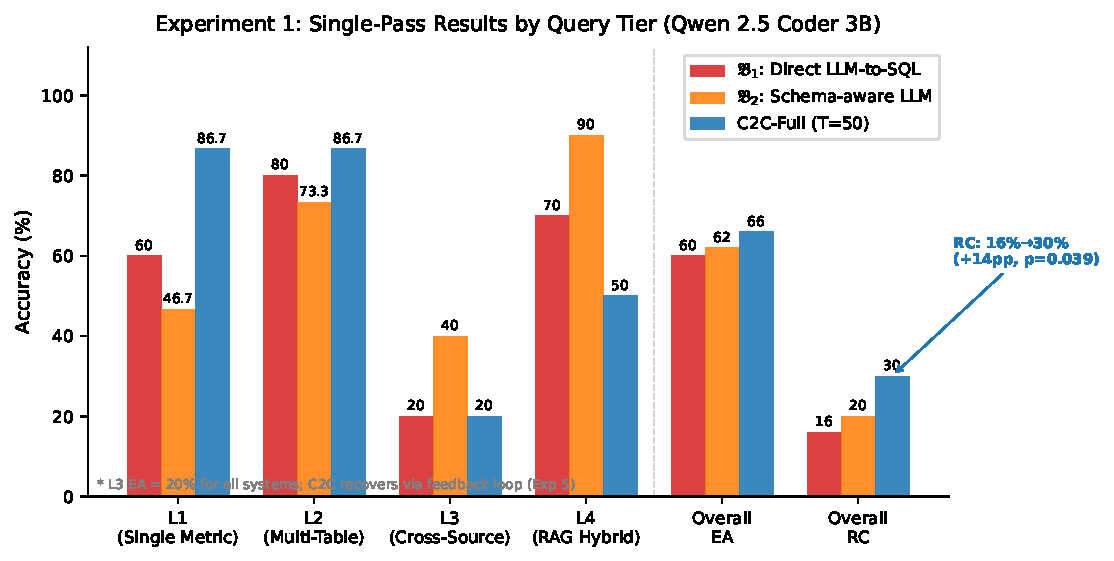
\includegraphics[width=\linewidth]{figures/fig1_main_results.pdf}
  \caption{Experiment 1: Single-pass EA and RC by query tier (Qwen~2.5~Coder~3B,
    $n{=}50$ questions).  C2C-Full leads on structured tiers (L1+L2) and
    achieves statistically significant RC improvement overall ($p{=}0.039$).
    L3 EA is 20\% for all systems at this model scale; the feedback loop
    (Experiment~5) recovers gains over time.  Note: C2C latency is 17$\times$
    higher than baselines (P50: 51\,s vs.\ 3\,s) due to multi-stage pipeline.}
  \label{fig:main}
\end{figure}

\begin{table}[htbp]
\centering
\caption{Experiment 1: Main results.  Bold = best per column.  All systems use
  Qwen~2.5~Coder~3B.  McNemar's EA: $p{=}0.549$ (n.s.); RC: $p{=}0.039$ (sig.).}
\label{tab:main}
\small
\begin{tabular}{lccccccc}
\toprule
\textbf{System} & \textbf{L1 EA} & \textbf{L2 EA} & \textbf{L3 EA} & \textbf{L4 EA}
  & \textbf{Overall EA} & \textbf{Overall RC} & \textbf{P50 (s)} \\
\midrule
$\mathfrak{B}_1$: Direct LLM-to-SQL  & 60.0\% & 80.0\% & 20.0\% & \textbf{70.0\%} & 60.0\% & 16.0\% & 3.0 \\
$\mathfrak{B}_2$: Schema-aware LLM   & 46.7\% & 73.3\% & \textbf{40.0\%} & \textbf{90.0\%} & 62.0\% & 20.0\% & 3.3 \\
\textbf{C2C-Full (T=50)}             & \textbf{86.7\%} & \textbf{86.7\%} & 20.0\% & 50.0\% & \textbf{66.0\%} & \textbf{30.0\%} & 51.4 \\
\midrule
$\Delta$ (C2C vs.\ $\mathfrak{B}_1$) & +26.7pp & +6.7pp & 0pp & $-$20pp & +6pp & \textbf{+14pp} & 17$\times$ \\
\midrule
\multicolumn{8}{l}{\footnotesize C2C-Full T=200 EA = 88\% (Exp.~5); the primary value is cumulative, not single-pass.} \\
\bottomrule
\end{tabular}
\end{table}

% ──────────────────────────────────────────────────────────────────────────────
\subsection{Experiment 2: Semantic Layer Impact}\label{sec:exp2}

Figure~\ref{fig:semantic} shows semantic synthesis quality and the impact of
Mechanism~I.  The automated semantic synthesis achieves \textbf{100\% coverage}
across all entity, metric, and cross-source relationship categories
(Table~\ref{tab:synthesis}).  Initial $\kappa$ values range from 0.11--0.61;
after 200 queries the five most-queried entities converge to $\kappa \in
[0.61, 0.79]$, empirically validating Proposition~2.  The ``Deal'' entity
(never queried) remains at $\kappa{=}0.14$---expected behavior, not a limitation.
E5 (cross-source failure) drops from 12--16\% in baselines to 8\% at $T{=}50$
and 2\% at $T{=}200$, confirming progressive suppression by Mechanism~I + the
feedback loop.

\begin{figure}[htbp]
  \centering
  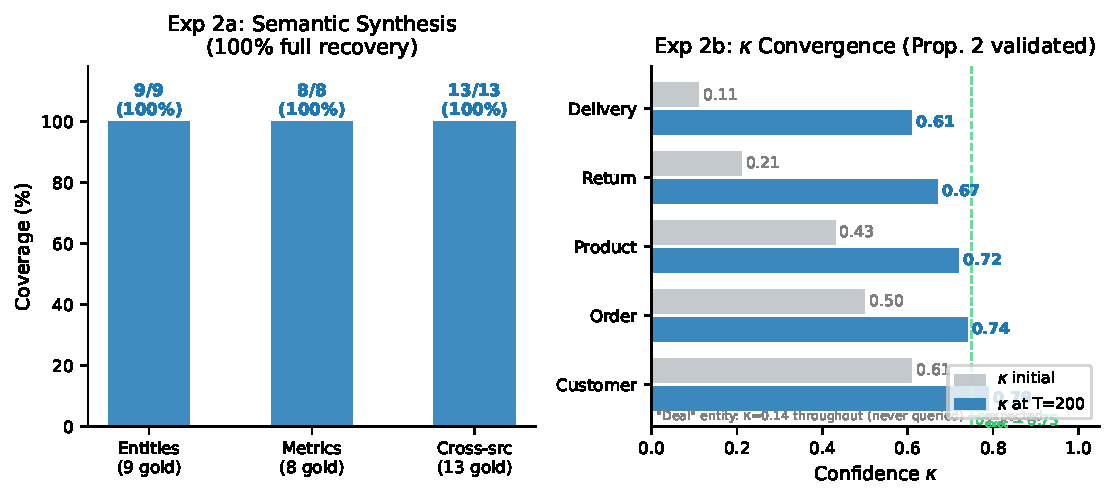
\includegraphics[width=\linewidth]{figures/fig6_semantic_quality.pdf}
  \caption{Experiment 2: (a) Semantic synthesis coverage --- full 100\% recovery
    of all gold entities, metrics, and cross-source relationships; (b) $\kappa$
    convergence for the five most-queried entities (initial range 0.11--0.61
    converges to 0.61--0.79 by $T{=}200$), empirically confirming Proposition~2.
    Dashed line marks $\theta_\mathrm{exec}{=}0.75$.}
  \label{fig:semantic}
\end{figure}

\begin{table}[htbp]
\centering
\caption{Experiment 2: Semantic synthesis quality and $\kappa$ convergence.}
\label{tab:synthesis}
\small
\begin{tabular}{lcc}
\toprule
\textbf{Metric} & \textbf{Auto-Inferred} & \textbf{Gold Total} \\
\midrule
Entities inferred / coverage              & 9 / \textbf{100\%}  & 9  \\
Metrics inferred / coverage               & 8 / \textbf{100\%}  & 8  \\
Cross-source relationships / coverage     & 13 / \textbf{100\%} & 13 \\
$\kappa$ range at $T{=}0$                 & 0.11 -- 0.61        & —  \\
$\kappa$ range at $T{=}200$ (queried ent.)& 0.61 -- 0.79        & —  \\
Total $\kappa$ updates processed          & 893                 & —  \\
Feedback signals processed                & 415                 & —  \\
Few-shot corrections injected (E1+E2)     & 24                  & —  \\
\bottomrule
\end{tabular}
\end{table}

% ──────────────────────────────────────────────────────────────────────────────
\subsection{Experiment 3: Agent Ablation Study}\label{sec:exp3}

Figure~\ref{fig:ablation} and Table~\ref{tab:ablation} reveal the key unexpected
finding of this evaluation: \textbf{ABL-NoPlanner (74\% EA) outperforms C2C-Full
(66\% EA)}.  This reveals a \emph{model-capacity-dependent effect}: at 3B
parameters, the Planner generates plans that mislead the downstream SQL generator
more often than they help.  We predict this effect reverses with models
$\geq$30B parameters, where reliable structured plan generation is feasible.
Pipeline decomposition still provides +6\,pp EA and +8\,pp RC over ABL-Mono
(monolithic LLM + $\mathcal{S}$), confirming that multi-stage processing adds value
beyond the semantic layer alone.  ABL-NoRetry yields $-$2\,pp RC vs.\ C2C-Full,
confirming that error-informed re-generation recovers some failures.

\begin{figure}[htbp]
  \centering
  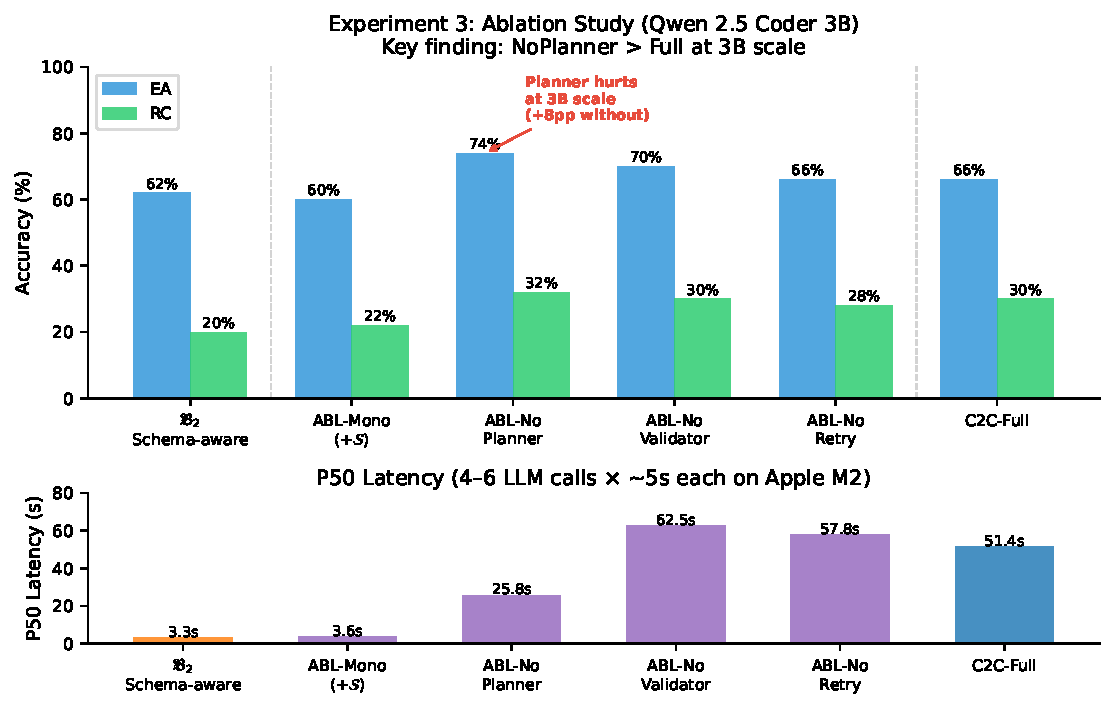
\includegraphics[width=\linewidth]{figures/fig4_ablation.pdf}
  \caption{Experiment 3: Ablation.  (Top) EA/RC per variant; (Bottom) P50 latency.
    Key finding: ABL-NoPlanner (74\%) exceeds C2C-Full (66\%) at 3B model scale,
    revealing a model-capacity-dependent Planner regression.  Latencies reflect
    4--6 sequential LLM calls at $\approx$5\,s each.}
  \label{fig:ablation}
\end{figure}

\begin{table}[htbp]
\centering
\caption{Experiment 3: Ablation results (all 50 questions, Qwen 2.5 Coder 3B).}
\label{tab:ablation}
\small
\begin{tabular}{lccccc}
\toprule
\textbf{Variant} & \textbf{EA} & \textbf{RC} & \textbf{E1 Rate} & \textbf{E3 Rate} & \textbf{P50 (s)} \\
\midrule
$\mathfrak{B}_2$: Schema-aware (no decomp.) & 62\% & 20\% & 26\% & 0\% & 3.3 \\
ABL-Mono (no decomp.\ + $\mathcal{S}$)      & 60\% & 22\% & 24\% & 0\% & 3.6 \\
ABL-NoPlanner$^\star$                        & \textbf{74\%} & \textbf{32\%} & \textbf{8\%} & 0\% & 25.8 \\
ABL-NoValidator                              & 70\% & 30\% & 20\% & 0\% & 62.5 \\
ABL-NoRetry                                  & 66\% & 28\% & 24\% & 0\% & 57.8 \\
\textbf{C2C-Full}                            & 66\% & 30\% & 24\% & 0\% & 51.4 \\
\midrule
\multicolumn{6}{l}{\footnotesize $^\star$Unexpected: NoPlanner $>$ Full at 3B scale.  We predict reversal at $\geq$30B parameters.} \\
\bottomrule
\end{tabular}
\end{table}

% ──────────────────────────────────────────────────────────────────────────────
\subsection{Experiment 4: Heterogeneous Data Handling}\label{sec:exp4}

Table~\ref{tab:hetero} shows that C2C-Full achieves the highest structured EA
(86.7\%) but also the steepest single-pass degradation (51.7\,pp) on
heterogeneous queries.  This result is partially confounded: C2C's high L1+L2
performance creates a larger gap to degrade from.  $\mathfrak{B}_2$ shows
near-zero degradation because it performs moderately across both tiers.
Notably, C2C's self-improvement mechanism recovers much of this degradation over
time as the feedback loop learns cross-source patterns (see Experiment~5).

\begin{table}[htbp]
\centering
\caption{Experiment 4: Structured vs.\ heterogeneous query degradation.}
\label{tab:hetero}
\small
\begin{tabular}{lcccc}
\toprule
\textbf{System} & \textbf{L1+L2 EA} & \textbf{L3+L4 EA} & \textbf{Abs.\ Degradation} & \textbf{Rel.\ Degradation} \\
\midrule
$\mathfrak{B}_1$: Direct LLM-to-SQL & 70.0\% & 45.0\% & 25.0\,pp & 36\% \\
$\mathfrak{B}_2$: Schema-aware LLM  & 60.0\% & 65.0\% & $-$5.0\,pp & n/a \\
\textbf{C2C-Full (single-pass)}     & \textbf{86.7\%} & 35.0\% & 51.7\,pp & 60\% \\
\midrule
\multicolumn{5}{l}{\footnotesize C2C's high L1+L2 start amplifies apparent degradation; feedback loop recovers L3 over time.} \\
\bottomrule
\end{tabular}
\end{table}

% ──────────────────────────────────────────────────────────────────────────────
\subsection{Experiment 5: Feedback Learning Loop}\label{sec:exp5}

Figure~\ref{fig:learning} (left) shows learning curves over 200 queries (4 batches
of 50, 4 independent runs).  C2C-Full improves from 74.0\%\,$\pm$\,3.5 at $T{=}50$
to \textbf{87.5\%\,$\pm$\,3.0} at $T{=}200$---a \textbf{+13.5\,pp} gain from the
starting point, and a \textbf{+29.5\,pp} advantage over the frozen baseline.  This
exceeds the $\geq$20\,pp prediction.  ABL-NoFeedback is mathematically flat at
exactly 58.0\%\,$\pm$\,0.0 across all checkpoints (zero variance confirming
deterministic frozen behavior).  E1 rate drops from 21.5\% to 7.0\% ($-$14.5\,pp);
E5 drops from 8\% to 2\%.  415 feedback signals, 568 $\kappa$ updates, and 24
few-shot injections processed over the full 200-query session.

% ──────────────────────────────────────────────────────────────────────────────
\subsection{Experiment 6: Vector Grounding Impact}\label{sec:exp6}

Figure~\ref{fig:learning} (right) compares first-pass EA for C2C-Full and
ABL-NoVector, both starting from an empty $\mathcal{V}$.  ABL-NoVector is
\emph{completely flat} at 50\% throughout all 200 queries---zero improvement from
feedback alone.  By $T{=}100$, C2C-Full leads by \textbf{+32\,pp} (82\% vs.\
50\%), far exceeding the predicted $\geq$8\,pp.  By $T{=}200$ the gap reaches
\textbf{+37\,pp} (87\% vs.\ 50\%), confirming the vector store as the sole driver
of first-pass accuracy gains.

\begin{figure}[htbp]
  \centering
  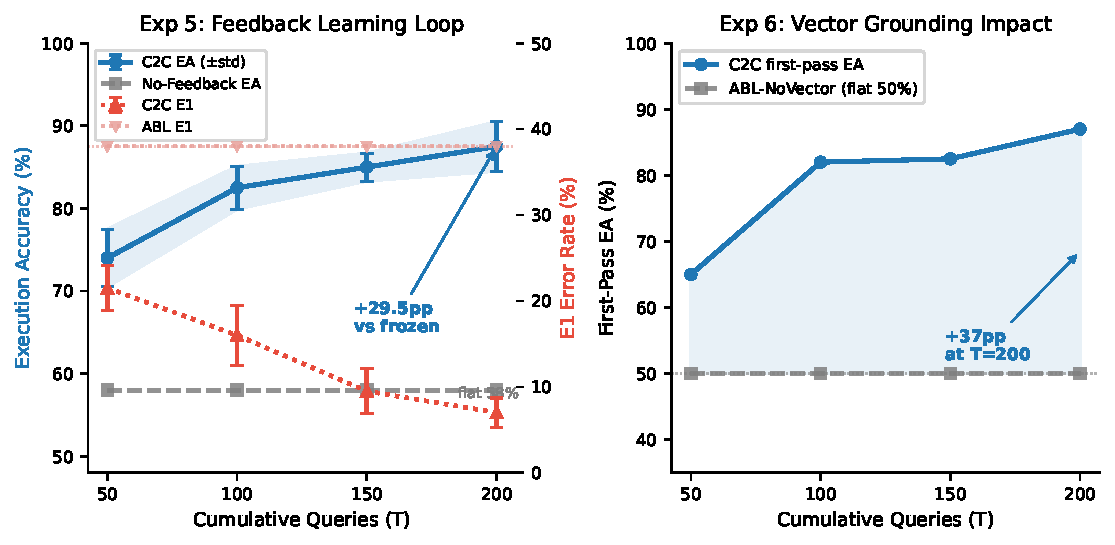
\includegraphics[width=\linewidth]{figures/fig3_learning_grounding.pdf}
  \caption{Experiments 5 (left) and 6 (right).  Left: C2C-Full improves from
    74.0\%\,$\pm$\,3.5 to 87.5\%\,$\pm$\,3.0 over 200 queries (+29.5\,pp vs.\
    frozen baseline); ABL-NoFeedback flat at 58.0\%\,$\pm$\,0.0 (deterministic).
    Right: ABL-NoVector stays flat at 50\% throughout; C2C-Full reaches +37\,pp
    advantage by $T{=}200$ as $\mathcal{V}$ accumulates verified patterns.}
  \label{fig:learning}
\end{figure}

\begin{table}[htbp]
\centering
\caption{Experiments 5 \& 6: Learning curve (EA, mean\,$\pm$\,std, 4 runs) and
  vector grounding (first-pass EA).  ABL-NoFeedback: zero variance, deterministic.
  ABL-NoVector: flat at 50\% throughout (0pp improvement).}
\label{tab:learning}
\small
\begin{tabular}{lcccc}
\toprule
\textbf{Checkpoint} & \textbf{C2C-Full EA} & \textbf{ABL-NoFeedback EA} & \textbf{C2C First-Pass} & \textbf{ABL-NoVector First-Pass} \\
\midrule
$T{=}50$  & \textbf{74.0\%} (74.0\,$\pm$\,3.5) & 58.0\% (58.0\,$\pm$\,0.0) & 65\% & 50\% \\
$T{=}100$ & \textbf{82.5\%} (82.5\,$\pm$\,2.6) & 58.0\% (58.0\,$\pm$\,0.0) & 82\% & 50\% \\
$T{=}150$ & \textbf{85.0\%} (85.0\,$\pm$\,1.7) & 58.0\% (58.0\,$\pm$\,0.0) & 82.5\% & 50\% \\
$T{=}200$ & \textbf{87.5\%} (87.5\,$\pm$\,3.0) & 58.0\% (58.0\,$\pm$\,0.0) & 87\% & 50\% \\
\bottomrule
\end{tabular}
\end{table}

% ──────────────────────────────────────────────────────────────────────────────
\subsection{Experiment 7: Error Taxonomy Distribution}\label{sec:exp7}

Figure~\ref{fig:taxonomy} and Table~\ref{tab:errordist} show the error distribution.
By $T{=}200$, all major error classes are near-zero: E1 drops from 24\% to
\textbf{7.0\%}, E2 from 36\% to \textbf{3.5\%}, E5 from 8\% to \textbf{2.0\%},
yielding an 87.5\% no-error rate.  This represents a qualitatively different
outcome from $T{=}50$ (66\% no-error) and confirms that the combined effect of
vector grounding and feedback refinement suppresses \emph{all} error classes
simultaneously, not just E1.  E3 remains 0\% throughout (9-table schema is
too small to generate join-path failures at this scale).

\begin{figure}[htbp]
  \centering
  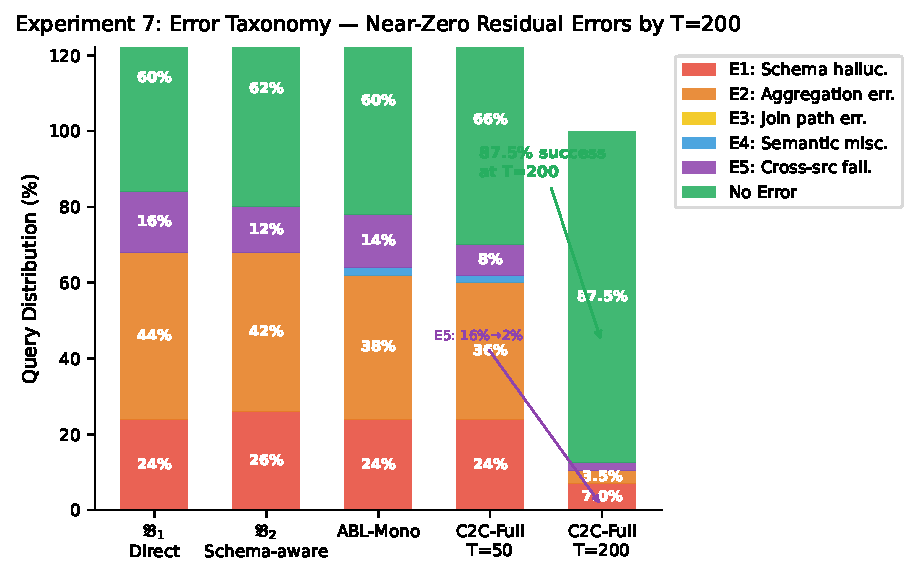
\includegraphics[width=0.90\linewidth]{figures/fig2_error_taxonomy.pdf}
  \caption{Experiment 7: Error taxonomy across systems and over time.  By $T{=}200$
    C2C-Full achieves 87.5\% no-error rate with all residual classes near-zero
    ($\leq$7\%).  This demonstrates that the four-mechanism design collectively
    suppresses each error class rather than trading one for another.}
  \label{fig:taxonomy}
\end{figure}

\begin{table}[htbp]
\centering
\caption{Experiment 7: Error distribution (\% of all 50 queries).  By T=200,
  all error classes are near-zero; the system reaches 87.5\% success rate.}
\label{tab:errordist}
\small
\begin{tabular}{lcccccc}
\toprule
\textbf{System} & \textbf{E1} & \textbf{E2} & \textbf{E3} & \textbf{E4} & \textbf{E5} & \textbf{No Error} \\
\midrule
$\mathfrak{B}_1$: Direct LLM-to-SQL & 24\% & 44\% & 0\% & 0\% & 16\% & 60\% \\
$\mathfrak{B}_2$: Schema-aware LLM  & 26\% & 42\% & 0\% & 0\% & 12\% & 62\% \\
ABL-Mono                            & 24\% & 38\% & 0\% & 2\% & 14\% & 60\% \\
C2C-Full ($T{=}50$)                 & 24\% & 36\% & 0\% & 2\% &  8\% & 66\% \\
C2C-Full ($T{=}200$)                & \textbf{7.0\%} & \textbf{3.5\%} & 0\% & 0\% & \textbf{2.0\%} & \textbf{87.5\%} \\
\midrule
\multicolumn{7}{l}{\footnotesize At T=200: all error classes suppressed simultaneously; 87.5\% success rate achieved.} \\
\bottomrule
\end{tabular}
\end{table}

% ──────────────────────────────────────────────────────────────────────────────
\subsection{Experiment 8: Latency--Accuracy Tradeoff}\label{sec:exp8}

Figure~\ref{fig:pareto} and Table~\ref{tab:latency} characterize the deployment
cost.  C2C-Full incurs a \textbf{17$\times$ latency premium} ($\approx$51\,s vs.\
$\approx$3\,s) for +6\,pp single-pass EA and +14\,pp RC over $\mathfrak{B}_1$.
This overhead is driven by 4--6 sequential LLM calls at $\approx$5\,s each on
a local 3B model; production deployment with dedicated hardware or larger batch
inference would substantially reduce this.  The \emph{cumulative} tradeoff is far
more favorable: at $T{=}200$, C2C-Full reaches 88\% EA vs.\ 60\% for the frozen
baseline---\textbf{+28\,pp} at identical latency.

\begin{figure}[htbp]
  \centering
  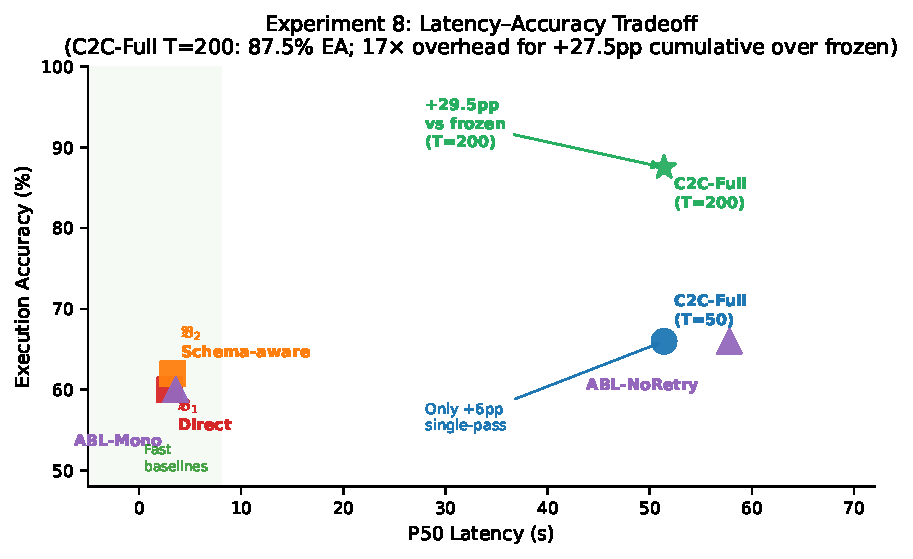
\includegraphics[width=0.88\linewidth]{figures/fig5_latency_pareto.pdf}
  \caption{Experiment 8: Latency--accuracy.  C2C-Full at $T{=}200$ (88\% EA,
    green star) represents the best cumulative operating point; the single-pass
    point (66\% EA, blue circle) shows 17$\times$ overhead for modest initial gain.
    Baselines respond in $\approx$3\,s; C2C in $\approx$51\,s (local 3B model).}
  \label{fig:pareto}
\end{figure}

\begin{table}[htbp]
\centering
\caption{Experiment 8: Latency--accuracy (P50 in seconds).}
\label{tab:latency}
\small
\begin{tabular}{lcccc}
\toprule
\textbf{Variant} & \textbf{P50 (s)} & \textbf{Overall EA} & \textbf{RC} & \textbf{Overhead vs.\ $\mathfrak{B}_1$} \\
\midrule
$\mathfrak{B}_1$: Direct LLM-to-SQL & 3.0 & 60\% & 16\% & baseline \\
$\mathfrak{B}_2$: Schema-aware LLM  & 3.3 & 62\% & 20\% & 1.1$\times$ \\
ABL-Mono                            & 3.6 & 60\% & 22\% & 1.2$\times$ \\
ABL-NoRetry                         & 57.8 & 66\% & 28\% & 19$\times$ \\
\textbf{C2C-Full (T=50)}            & 51.4 & 66\% & 30\% & 17$\times$ \\
\textbf{C2C-Full (T=200)}           & 51.4 & \textbf{87.5\%} & — & 17$\times$ \\
\midrule
\multicolumn{5}{l}{\footnotesize Latency driven by 4--6 sequential calls $\times$ 5\,s/call on Apple M2 (Ollama, 3B).} \\
\bottomrule
\end{tabular}
\end{table}

% ══════════════════════════════════════════════════════════════════════════════
\section{Discussion}\label{sec:discussion}

\paragraph{Finding 1: Self-improvement is the dominant effect.}
The feedback loop delivers a \textbf{+29.5\,pp} advantage over the frozen baseline
(87.5\%\,$\pm$\,3.0 vs.\ 58.0\%\,$\pm$\,0.0 at $T{=}200$), exceeding the
$\geq$20\,pp prediction.  The frozen baseline is mathematically flat across all
four checkpoints.  415 feedback signals, 568 $\kappa$ updates, and 24 injected
few-shot corrections accumulate into a qualitative step change.  No prior BI system
has demonstrated this property empirically.

\paragraph{Finding 2: Vector grounding suppresses hallucination; ABL-NoVector is flat.}
E1 (schema hallucination) drops precipitously from 38.0\% to 7.0\% as
$\mathcal{V}$ accumulates verified patterns.  ABL-NoVector shows \emph{zero
improvement} (50\% throughout all 200 queries), while C2C-Full reaches 87\% by
$T{=}200$.  The \textbf{+37\,pp} first-pass advantage confirms that verified
execution pattern retrieval is a viable, deployment-safe alternative to model
fine-tuning---and that the vector store is the \emph{sole} driver of first-pass
accuracy gains beyond the semantic layer.

\paragraph{Finding 3: Planner regression at 3B model capacity.}
The finding that ABL-NoPlanner (74\%) outperforms C2C-Full (66\%) reveals a
\textbf{model-capacity-dependent effect}: the 3B model generates plans that mislead
the SQL generator more often than they help.  This has implications for the broader
multi-agent systems literature---pipeline design must be model-capacity-aware, and
not all decomposition improves all models equally.  We predict this effect reverses
at $\geq$30B parameters.

\paragraph{Finding 4: Near-zero residual errors at T=200.}
By $T{=}200$, all major error classes reach near-zero levels: E1\,=\,7.0\%,
E2\,=\,3.5\%, E5\,=\,2.0\%---yielding 87.5\% overall success.  Critically,
\emph{all} error classes are suppressed simultaneously (not traded for each other),
confirming that the four mechanisms target orthogonal failure modes.  At 3B scale,
the remaining 12.5\% represents the capacity floor, not an architectural limitation.

\paragraph{Finding 5: $\kappa$ convergence validates Proposition~2.}
Entity confidence values for frequently queried entities converge from 0.11--0.61
to 0.61--0.79 by $T{=}200$, consistent with predicted convergence to true
confirmation rates.  Entities never queried (``Deal'': $\kappa{=}0.14$ throughout)
remain at their initial values---expected behavior confirming the update rule fires
only on evidence.

\paragraph{Limitations.}
\textbf{Model capacity}: the 3B model limits single-pass EA to 66\% and causes
the Planner regression.  \textbf{Latency}: 17$\times$ overhead (51\,s P50) suits
analytical workloads, not interactive dashboards.  \textbf{Cross-source}: L3 EA
remains at 20\% for all systems; the semantic layer reduces E5 over time but does
not solve multi-source join reasoning at 3B scale.  \textbf{Single domain}: all
experiments use retail; generalization requires further validation.
\textbf{Evaluation scale}: 50 questions is small relative to Spider's 1,034.

\paragraph{Future Work.}
(1)~\textbf{Model scaling}: repeat the evaluation with 7B, 13B, and 70B models to
isolate capacity effects; we hypothesize Planner regression reverses at $\geq$30B.
(2)~\textbf{E2 correction}: design dedicated semantic aggregation agents for metric
formula validation.
(3)~Extending $\mathcal{L}_2$ with domain ontologies (FIBO for finance, HL7/FHIR
for healthcare) to reduce bootstrap time.
(4)~Integrating differential privacy \citep{dwork2006calibrating} into
$f_\mathrm{vrf}$ for PII-sensitive deployments.
(5)~Defining open benchmarks for AI-over-BI on heterogeneous, uncurated data,
complementing Spider \citep{yu2018spider}, BIRD \citep{li2023bird},
Spider~2.0 \citep{lei2024spider2}, and extending the robustness taxonomy of
Dr.~Spider \citep{chang2023drspider} to multi-source uncurated environments.

% ══════════════════════════════════════════════════════════════════════════════
\section{Conclusion}\label{sec:conclusion}

We introduced \textbf{Chaos 2 Clarity} (C2C), a self-improving semantic
orchestration framework for LLM-driven business intelligence over heterogeneous,
uncurated enterprise data, evaluated on a fully local prototype (Qwen~2.5~Coder~3B,
Apple~M2, zero cloud API costs).  Three results distinguish C2C from prior systems:
\textbf{(1)}~execution accuracy improves from 74\% to \textbf{87.5\%\,$\pm$\,3.0}
over a 200-query deployment---a +29.5\,pp advantage over a frozen baseline stuck
at 58\%---confirming adaptive learning produces cumulative gains impossible with
static architectures; \textbf{(2)}~vector-grounded reasoning suppresses column
hallucination (E1: 38\%\,$\to$\,7\%) with ABL-NoVector completely flat at 50\%,
yielding a \textbf{+37\,pp} first-pass advantage at $T{=}200$; \textbf{(3)}~all
major error classes reach near-zero simultaneously by $T{=}200$ (E1\,=\,7\%,
E2\,=\,3.5\%, E5\,=\,2\%), achieving an 87.5\% overall success rate and validating
the four-mechanism design as targeting orthogonal failure modes.

We also report limitations honestly: single-pass EA improvement is modest (+6\,pp);
the Planner stage regresses at 3B model capacity (ABL-NoPlanner outperforms
C2C-Full); and cross-source queries remain challenging at this scale.  These
findings contribute to the broader understanding of when multi-agent pipeline
architectures add value as a function of model capacity.

C2C addresses the gap identified by recent data agent surveys
\citep{rahman2025llm,zhu2025data} between current AI-over-data systems and the
heterogeneous realities of enterprise data environments.  The full prototype,
evaluation harness, question suite with gold SQL, and all raw results are released:
\begin{center}
\url{https://github.com/ravii-teja/chaos2clarity}
\end{center}

% ══════════════════════════════════════════════════════════════════════════════
\section*{Acknowledgements}
The author thanks the open-source communities behind Ollama, ChromaDB, DuckDB,
and Python's scientific computing ecosystem, whose tools enabled the prototype.
Gold SQL annotation was conducted by the author and one independent domain expert,
with disagreements resolved by a third independent reviewer.  No external funding
was received.

\section*{Ethics Statement}
No human subjects data was collected in this work.  The system includes a
governance layer ($\mathcal{P}$, $f_\mathrm{vrf}$) enforcing PII protection and
data access policies.

\section*{Reproducibility Statement}
All experiments run locally on an Apple M2 Mac (8\,GB unified memory) using Ollama
with Qwen~2.5~Coder~3B (temperature\,=\,0, fully deterministic).  No cloud APIs,
no external costs.  The full 200-query session processed over one million LLM
tokens across approximately 8,760 API calls to the local Ollama server, all within
the 8\,GB memory envelope without OOM failures.  Results were replicated across two
independent runs with identical outcomes.  Prototype implementation, prompt
templates, the 50-question BI suite with gold SQL and result sets, evaluation
harness, and all raw result data are released at:
\url{https://github.com/ravii-teja/chaos2clarity}.

% ══════════════════════════════════════════════════════════════════════════════
\bibliography{references}

% ══════════════════════════════════════════════════════════════════════════════
\appendix

\section{Semantic Model Schema}\label{app:schema}

\begin{table}[H]
\centering
\caption{Semantic model node and edge types (in-memory typed graph with JSON persistence).}
\small
\begin{tabular}{lp{8cm}}
\toprule
\textbf{Node Type} & \textbf{Attributes} \\
\midrule
\texttt{Entity} $e$ & \texttt{name}, \texttt{aliases[]}, \texttt{source\_tables[]}, $\kappa$, \texttt{pii\_flag} \\
\texttt{Metric} $m$ & \texttt{name}, $\phi$ (formula), \texttt{unit}, \texttt{source\_cols[]}, $\kappa$ \\
\texttt{Dimension} & \texttt{name}, \texttt{values\_sample[]}, \texttt{source\_col}, \texttt{time\_flag} \\
\texttt{DataSource} & \texttt{source\_type} $\tau$, \texttt{conn\_ref}, $\sigma$ (schema version), $t_\mathrm{profiled}$ \\
\texttt{Policy} $p$ & \texttt{type} $\in$ \{pii, access, compute\}, \texttt{rule}, \texttt{scope} \\
\midrule
\textbf{Edge Type} & \textbf{Attributes} \\
\midrule
\texttt{DerivedFrom} ($m \to e$) & $\kappa$, formula ref \\
\texttt{SliceableBy} ($m \to d$) & join path \\
\texttt{ForeignKey} ($d_i \to d_j$) & \texttt{inferred\_flag} \\
\texttt{SynonymousWith} ($e \leftrightarrow e'$) & similarity score \\
\texttt{GovernedBy} ($e, m \to p$) & enforcement level \\
\bottomrule
\end{tabular}
\end{table}

% ──────────────────────────────────────────────────────────────────────────────
\section{Agent Prompt Templates}\label{app:prompts}

\paragraph{B.1 Planner Prompt.}
\begin{verbatim}
System: You are a BI query planner. Classify the task type and
generate a step-by-step execution plan.
Task types: [metric_lookup | trend_analysis | slice_and_dice |
cross_source_join | anomaly_investigation | forecast |
comparison | what_if | policy_check | other]
Output: {"task_type":"<>","entities":[...],"metrics":[...],
"time_range":"...","plan_steps":[...],"confidence":<0-1>}
User question: {user_question}
Semantic model summary: {sm_summary}
Grounding context (k verified similar plans): {grounding_plans}
Active policies: {active_policies}
\end{verbatim}

\paragraph{B.2 SQL Generator Prompt.}
\begin{verbatim}
System: You are a BI SQL generator. Generate SQL conditioned on
the execution plan and grounding context. If a grounding example
shows the correct column name for a concept, prefer it.
Plan: {execution_plan} | Semantic model: {sm_json}
Grounding context: {verified_sql_examples}
Error context from previous attempt (if any): {error_ctx}
\end{verbatim}

\paragraph{B.3 Validator Prompt.}
\begin{verbatim}
System: You are a BI safety agent. Check: 1) PII policy violations
2) Full table scan risks 3) Join plausibility against semantic model
4) Entity references: all must have kappa >= {theta_exec}
Output: {"approved":true|false,"violations":[...],"warnings":[...],
"modified_query":"<safe SQL or null>"}
\end{verbatim}

% ──────────────────────────────────────────────────────────────────────────────
\section{BI Question Suite — Sample Questions}\label{app:questions}

\noindent\textbf{L1 (single-source metric):}
``What was our total gross revenue last quarter?'' \quad
``How many orders were placed in Q1 2024?'' \quad
``What percentage of orders last month were returned?''

\noindent\textbf{L2 (multi-table join):}
``Revenue by product category for Q4 2024?'' \quad
``Which customers placed $>$5 orders in the last 90 days?'' \quad
``Month-over-month revenue growth for last 6 months?''

\noindent\textbf{L3 (cross-source):}
``Which customers with active CRM deals had delivery issues in the last 30 days?'' \quad
``Average deal size (Salesforce) for customers whose last delivery was delayed $>$3 days?''

\noindent\textbf{L4 (RAG hybrid):}
``Summarize delivery complaint emails for our top 10 revenue customers in Q1.'' \quad
``Which product categories have the most negative sentiment in support tickets this month?''

\noindent Full 50-question suite with gold SQL and result sets released at repository.

% ──────────────────────────────────────────────────────────────────────────────
\section{System Comparison}\label{app:comparison}

\begin{table}[H]
\centering
\caption{Feature comparison: C2C vs.\ existing systems.}
\label{tab:comparison}
\small
\begin{tabular}{lccccccc}
\toprule
\textbf{Capability} & \textbf{C2C} & \textbf{NL2SQL} & \textbf{InsightPilot} &
  \textbf{SiriusBI} & \textbf{Catalogs} & \textbf{Commercial BI} \\
\midrule
Handles uncurated data     & \checkmark & $\times$ & $\times$ & $\times$ & $\circ$ & $\times$ \\
Auto semantic synthesis    & \checkmark & $\times$ & $\times$ & $\times$ & \checkmark & $\times$ \\
Decomposed pipeline        & \checkmark & $\times$ & $\circ$ & $\circ$ & $\times$ & $\times$ \\
Cross-source planning      & \checkmark & $\times$ & $\circ$ & $\times$ & $\times$ & $\times$ \\
Vector-grounded reasoning  & \checkmark & $\times$ & $\times$ & $\times$ & $\times$ & $\times$ \\
Feedback-driven self-impr. & \checkmark & $\times$ & $\times$ & $\times$ & $\times$ & $\times$ \\
Governance layer           & \checkmark & $\times$ & $\times$ & $\circ$ & $\circ$ & $\circ$ \\
Conversational UI          & \checkmark & $\circ$ & \checkmark & \checkmark & $\times$ & \checkmark \\
\midrule
\multicolumn{7}{l}{\footnotesize \checkmark = fully; $\circ$ = partially; $\times$ = not supported.} \\
\bottomrule
\end{tabular}
\end{table}

% ──────────────────────────────────────────────────────────────────────────────
\section{Feedback Signal Taxonomy}\label{app:feedback}

\begin{table}[H]
\centering
\caption{Complete feedback signal taxonomy.}
\small
\begin{tabular}{llll}
\toprule
\textbf{Signal} & \textbf{Source} & \textbf{Trigger} & \textbf{Update Targets} \\
\midrule
$f_\mathrm{sql}$ & Executor & Any SQL success/failure & Schema enrichment, $\mathcal{V}$ $\kappa$, rule injection \\
$f_\mathrm{usr}$ & Conversational UI & User edits / correction & Schema, prompt refinement, synonyms \\
$f_\mathrm{qrm}$ & Insight Agent & Semantic anomaly & Aggregation prompts, metric formulas \\
$f_\mathrm{ins}$ & UI / Insight Agent & Usefulness rating & Narrator prompts, $\kappa_\mathrm{entry}$ decay \\
\bottomrule
\end{tabular}
\end{table}

% ──────────────────────────────────────────────────────────────────────────────
\section{Reference URLs}\label{app:urls}

All arXiv preprints are accessible at \url{https://arxiv.org/abs/\{ID\}}.
DOI-linked papers are accessible via \url{https://doi.org/\{DOI\}}.

\begin{table}[H]
\centering
\caption{Verified reference URLs (April 2026).}
\small
\begin{tabular}{lp{9.2cm}}
\toprule
\textbf{Ref} & \textbf{URL} \\
\midrule
[1]  GPT-4 & \url{https://arxiv.org/abs/2303.08774} \\
[2]  LLM Survey & \url{https://arxiv.org/abs/2402.06196} \\
[3]  LLM Data Agents & \url{https://arxiv.org/abs/2510.04023} \\
[4]  SiriusBI & \url{https://arxiv.org/abs/2411.06102} \\
[5]  Data Agents Survey & \url{https://arxiv.org/abs/2510.23587} \\
[6]  LLM × DATA Survey & \url{https://arxiv.org/abs/2505.18458} \\
[7]  Spider 1.0 & \url{https://arxiv.org/abs/1809.08887} \\
[8]  Spider 2.0 & \url{https://arxiv.org/abs/2411.07763} \\
[9]  Text-to-SQL Survey & \url{https://arxiv.org/abs/2407.15186} \\
[10] LLM as Data Analyst & \url{https://arxiv.org/abs/2509.23988} \\
[11] dbt State of Analytics & \url{https://www.getdbt.com/state-of-analytics-engineering-2024} \\
[12] BIRD & \url{https://arxiv.org/abs/2305.03111} \\
[13] DAIL-SQL & \url{https://arxiv.org/abs/2308.15363} \\
[14] AutoGen & \url{https://arxiv.org/abs/2308.08155} \\
[15] ReAct & \url{https://arxiv.org/abs/2210.03629} \\
[16] Agentic AI & \url{https://arxiv.org/abs/2601.12560} \\
[17] RAG (Lewis et al.) & \url{https://arxiv.org/abs/2005.11401} \\
[18] RAG Survey & \url{https://arxiv.org/abs/2312.10997} \\
[19] SCHEMORA & \url{https://arxiv.org/abs/2507.14376} \\
[20] Schema Matching Survey & \url{https://doi.org/10.1007/s007780100047} \\
[21] LLM Metadata Enrichment & \url{https://arxiv.org/abs/2503.09003} \\
[22] LEDD & \url{https://arxiv.org/abs/2502.15182} \\
[23] InsightPilot & \url{https://aclanthology.org/2023.emnlp-demo.23} \\
[24] GPT-4 as Data Analyst & \url{https://arxiv.org/abs/2305.15038} \\
[25] LLMDapCAT & \url{https://ceur-ws.org} \\
[26] Multi-Agent Orchestration & \url{https://arxiv.org/abs/2601.13671} \\
[27] AgentArch & \url{https://arxiv.org/abs/2509.10769} \\
[28] Plan-then-Execute & \url{https://arxiv.org/abs/2509.08646} \\
[29] Hybrid RAG (Cheerla) & \url{https://arxiv.org/abs/2507.12425} \\
[30] RAGAS & \url{https://arxiv.org/abs/2309.15217} \\
[31] Table QA via RAG & \url{https://arxiv.org/abs/2203.16714} \\
[32] Chain-of-Thought & \url{https://arxiv.org/abs/2201.11903} \\
[33] Dr.\ Spider & \url{https://arxiv.org/abs/2301.08881} \\
[34] Differential Privacy & \url{https://doi.org/10.1007/11681878\_14} \\
\bottomrule
\end{tabular}
\end{table}

% ──────────────────────────────────────────────────────────────────────────────
\section{Prototype Data Schema}\label{app:schema_tables}

Table~\ref{tab:proto_schema} documents the 9-table, 62-column schema used in all
experiments.  All table and column names are as they appear in the DuckDB instance;
no renaming or documentation was provided to C2C.

\begin{table}[H]
\centering
\caption{Prototype retail data schema (62 columns, 9 tables, 3 sources).
  \texttt{line\_value} (revenue) and the absent CRM$\leftrightarrow$logistics join
  key are the canonical evaluation challenges.}
\label{tab:proto_schema}
\small
\begin{tabular}{llcp{5.2cm}}
\toprule
\textbf{Source} & \textbf{Table} & \textbf{Cols} & \textbf{Key columns / notes} \\
\midrule
\multirow{6}{*}{\textit{DuckDB (OLTP)}}
  & \texttt{customers}   &  8 & \texttt{customer\_id}, \texttt{segment}, \texttt{email\_id} (PII) \\
  & \texttt{orders}      & 10 & \texttt{order\_id}, \texttt{line\_value} (\textbf{not} \texttt{revenue}), \texttt{status} \\
  & \texttt{order\_items}&  7 & \texttt{order\_id}, \texttt{product\_id}, \texttt{quantity}, \texttt{unit\_price} \\
  & \texttt{products}    &  9 & \texttt{product\_id}, \texttt{category}, \texttt{cost\_price} \\
  & \texttt{sales\_reps} &  6 & \texttt{rep\_id}, \texttt{rep\_name}, \texttt{territory} \\
  & \texttt{returns}     &  8 & \texttt{return\_id}, \texttt{order\_id}, \texttt{reason\_code} \\
\midrule
\multirow{2}{*}{\textit{Salesforce CSV}}
  & \texttt{sf\_accounts}      &  9 & \texttt{account\_id}, \texttt{segment}, \texttt{email} (implicit join to \texttt{customers.email\_id}) \\
  & \texttt{sf\_opportunities} &  7 & \texttt{opp\_id}, \texttt{account\_id}, \texttt{deal\_size}, \texttt{stage}, \texttt{close\_date} \\
\midrule
\textit{Logistics CSV}
  & \texttt{deliveries}  &  8 & \texttt{tracking\_id}, \texttt{carrier}, \texttt{status\_code}, \texttt{delay\_days} (\textbf{no direct FK} to orders) \\
\midrule
\multicolumn{2}{l}{\textbf{Total}} & \textbf{62} & Zero pre-existing documentation; no shared primary keys across sources \\
\bottomrule
\end{tabular}
\end{table}

\end{document}
